% Dokumentenkopf ---------------------------------------------------------------
%   Diese Vorlage basiert auf "scrreprt" aus dem koma-script.
% ------------------------------------------------------------------------------
%\documentclass[parskip=full-]{scrrprt}
	\documentclass[
	12pt, % Schriftgr��e
	DIV12,
	ngerman, % f�r Umlaute, Silbentrennung etc.
	a4paper, % Papierformat
	oneside, % einseitiges Dokument
	titlepage, % es wird eine Titelseite verwendet
	parskip=half, % Abstand zwischen Abs�tzen (halbe Zeile)
	headings=normal, % Gr��e der �berschriften verkleinern
	listof=totoc, % Verzeichnisse im Inhaltsverzeichnis auff�hren
	bibliography=totoc, % Literaturverzeichnis im Inhaltsverzeichnis auff�hren
	index=totoc, % Index im Inhaltsverzeichnis auff�hren
	captions=tableheading, % Beschriftung von Tabellen unterhalb ausgeben
	]{scrreprt}



\usepackage[
backend=biber,
style=alphabetic,
]{biblatex}

\usepackage{biblatex}
\addbibresource{ref.bib}

\usepackage{url}

\usepackage[
backend=biber,
style=alphabetic,
]{biblatex}

\usepackage{biblatex}
\addbibresource{ref.bib}

\usepackage{array}

\usepackage{listings}


\usepackage[utf8]{inputenc}
\usepackage{color}
\usepackage{textcomp}
\definecolor{bluekeywords}{rgb}{0,0,1}
\definecolor{greencomments}{rgb}{0,0.5,0}
\definecolor{redstrings}{rgb}{0.64,0.08,0.08}
\definecolor{xmlcomments}{rgb}{0.5,0.5,0.5}
\definecolor{types}{rgb}{0.17,0.57,0.68}
\usepackage{bookmark,hyperref}
\definecolor{lightgrey}{rgb}{0.95,0.95,0.95}
\lstset{language=[Sharp]C,
	captionpos=b,
	basicstyle=\fontfamily{consolas}\selectfont
	framextopmargin=26pt,
	tabsize=3,
	framexbottommargin=0pt, 
	frame=tb, framerule=0pt,
	showspaces=false,
	showtabs=false,
	breaklines=true,
	showstringspaces=false,
	breakatwhitespace=true,
	frame=single,
	backgroundcolor=\color{lightgrey},
	escapeinside={(*@}{@*)},
	commentstyle=\color{greencomments},
	morekeywords={partial, var, value, get, set, Action, Func, IEnumerable},
	keywordstyle=\color{bluekeywords},
	stringstyle=\color{redstrings},
	basicstyle=\ttfamily\small,
}
\usepackage[ngerman]{babel}
\usepackage{tabularx}
\usepackage{fixltx2e}
\usepackage{graphicx}
\usepackage{grffile}
\usepackage{longtable}
\usepackage{wrapfig}
\usepackage{rotating}


\usepackage[normalem]{ulem}
\usepackage{amsmath}
\usepackage{textcomp}
\usepackage{amssymb}
\usepackage{capt-of}
\usepackage{hyperref}
\usepackage[autostyle=true,german=quotes]{csquotes}
\let\svthefootnote\thefootnote
\newcommand\blankfootnote[1]{%
	\let\thefootnote\relax\footnotetext{#1}%
	\let\thefootnote\svthefootnote%
}

\date{\today}
\title{Flow Design}
\hypersetup{
	pdfauthor={},
	pdftitle={Flow Design},
	pdfkeywords={},
	pdfsubject={},
	pdfcreator={Emacs 25.1.1 (Org mode 8.3.5)}, 
	pdflang={German}}


\usepackage[T1]{fontenc}

\usepackage[german, refpage]{nomencl}
\makenomenclature
\let\abk\nomenclature 

\usepackage{listings}



\begin{document}

	\thispagestyle{empty}

\begin{center}
	

\large{Hochschule der Medien Stuttgart\\
Fakultät 1, Studiengang Medieninformatik}\\
\vspace{1cm}

\includegraphics[scale=1]{img/HdM-Logo.png}
\vspace{1.5cm}

\huge{Flow Design}

\large{Konzeption und Implementierung einer WPF Anwendung zur grafischen Modellierung und	Code-basierter Generierung von Flow Design Entwürfen unter Verwendung von C\# und Microsoft Roslyn}

\vspace{1cm}

\vspace{1cm}

\includegraphics[scale=0.07]{img/IT_DESIGNERS.jpg}
\vspace{1.5cm}

\large{
	Dennis Müller \\
	Matrikelnummer 25675\\
	9. Fachsemester\\
	dennis.briefkasten@gmail.com}

\vspace{3cm}
{24. Januar 2017}
\end{center}
	
	%TODO Ehrenwort
	
\chapter*{Ehrenwörtliche Erklärung}

Hiermit versichere ich, Dennis Müller, ehrenwörtlich, dass ich die vorliegende Bachelorarbeit  mit dem Titel: 

\begin{quote}
	Konzeption und Implementierung einer WPF-Anwendung zur grafischen
	Modellierung von Flow-Design-Entwürfen sowie Generierung von
	C\#-Code unter Verwendung von Microsoft Roslyn
\end{quote}


selbstständig und ohne fremde Hilfe verfasst und keine anderen als die angegebenen Hilfsmittel benutzt habe. Die Stellen der Arbeit, die dem Wortlaut oder dem Sinn nach anderen Werken entnommen wurden, sind in jedem Fall unter Angabe der Quelle kenntlich gemacht. Die Arbeit ist noch nicht veröffentlicht oder in anderer Form als Prüfungsleistung vorgelegt worden.

\vspace{0.5cm}

Ich habe die Bedeutung der ehrenwörtlichen Versicherung und die prüfungsrechtlichen Folgen (§ 24 Abs. 2 Bachelor-SPO der HdM) einer unrichtigen oder unvollständigen ehrenwörtlichen Versicherung zur Kenntnis genommen.
\vspace{1.5cm}

\titledate{Datum}



	
	%TODO Abstract
	\input{Inhalt/Abstract}	
	
	%TODO Danksagung
	
\chapter*{Danksagung}
Danke an Kevin Erath, der sich viel Zeit genommen hat, mir alles zu erklären und der mir 
die Flow Design Methodik näher gebracht hat.

Danke an Professor Walter Kriha für das Interesse an der Thematik, das hat mich zusätzlich motiviert eine 
gute Leistung zu bringen.

Danke auch Kevin Erath und Büsra für die Korrekturlesung.

Danke an die IT-Designer Gruppe für die finanzielle Unterstützung
und dafür, dass ich mich voll auf die Umsetzung meiner Bachelorarbeit konzentrieren konnte
und mir das nötige Arbeitsumfeld geboten hat.






	
	
	%%%%%%%%%%%%%%%%
	% Ab Inhaltsverzeichnis in diesem auch sichtbar
	%%%%%%%%%%%%%%%%		
	\tableofcontents

	
\chapter{Einführung}

\section{Motivation}

Software wird häufig einfach nur herunter-programmiert. Dadurch entsteht
umgangssprachlich bezeichnet Spaghetticode mit vielen Abhängigkeiten innerhalb
der eigenen Codebasis. Solch eine Codebasis ist schwer zu warten und auf
Änderungen anzupassen. Die Alternative dazu wäre, vor dem Programmieren einen
Entwurf der Architektur zu erstellen und sich vor der Umsetzung Gedanken zu
der Struktur zu machen.

Viele der vorhanden Entwurfsmethodiken sind jedoch zu schwergewichtig und helfen
einem nicht zwingend dabei Abhängigkeiten zu reduzieren.
Zusätzlich zu Entwurfsmethodiken existieren auch Clean Code Prinzipien, die
einem Helfen sollen, besser wartbare Software zu schreiben. Viele der
Erkenntnisse aus den Prinzipien sind jedoch leider oft nur schwer auf die eigene
Codebasis anzuwenden, da sie zu abstrakt sind.
Dadurch finden sie in der Praxis seltener Anwendung, als nötig wäre, um sauberen
Code zu schreiben.

Hier möchte Flow Design Abhilfe schaffen, indem sie eine leichtgewichtige
Entwurfsmethodik bietet, mit einem speziellen Augenmerk darauf Abhängigkeiten
zu reduzieren. Nebenbei hilft Flow Design einem auch gängige Clean Code
Prinzipien einzuhalten. 

Leider ist diese Methodik nicht weit verbreitet und das
Entwerfen ist bisher auf dem Papier angedacht. Aus diesem Grund existieren keine
ausgereiften Tools oder Hilfsprogramme die speziell auf die Erstellung
von Flow Design Entwürfen ausgelegt sind. 

Ziel dieser Arbeit ist es eine Anwendung zur Erstellung von Flow Design Diagrammen 
zu entwerfen und einen Prototypen zu implementieren. Diese Anwendung soll darüber hinaus auch
Funktionen zur Generierung von Quellcode aus den erstellten Diagrammen bieten, damit
der Einsatz von Flow Design in einem Projekt komfortabler und produktiver wird.

Unabhängig davon, ob dieses Ziel erreicht wurde oder nicht sollen die gewonnen
Erkenntnisse aus dem Versuch hier dokumentiert und ein Fazit daraus gezogen werden.

Der Prototyp soll in C\# und in Teilen unter Verwendung von Flow Design selbst umgesetzt und auf
Github als  Open-Source-Projekt veröffentlicht werden.



\section{Aufbau}

Der erste Teil dieser Arbeit stellt ein Grundlagenkapitel dar, dass dem Leser die Methodik Flow Design näher bringen soll.
Der Leser bekommt die Entwurfsmethodik Flow Design anschaulich erklärt, dabei wird auch auf die Herkunft,
den Grundgedanken dieser Methodik, sowie ihre Vor- und Nachteile eingegangen.
Dazu gehören auch, dass einige neue Prinzipien und Abkürzungen erklärt werden.
Des weiteren wird auf die für Flow Design speziellen, dazugehörigen Implemtierungsregeln eingegangen und
anhand von einfachen Codebeispielen in C\# dem Leser näher gebracht. 
Bei dieser Gelegenheit werden in diesem Teil auch auf einige Sprachfeatures 
von C\# eingegangen, die einem bei der Umsetzung von Datenströmen hilfreich sein
können. Auch hier werden einfache Codebeispiel zum besseren Verständnis dem Leser 
präsentiert. Im genauen handelt es sich hierbei um Lambdas und die Methodenbibliothek LINQ.

Hat man einmal den Vorteil von Flow Design für sich entdeckt liegt es nahe als
Programmierer sich Gedanken darüber zu machen wie eine Anwendung aussehen
könnte, das einem bei der Verwendung der Methodik so gut es geht unterstützt.
Da es solch ein Programm noch nicht gibt, geht es in diesem Teil der Arbeit
darum die Ansprüche eines solchen Programms im Detail herauszufinden und sie
in Form von Anforderungen aufzulisten. Anschließend werden GUI-Skizzen
und einige Gedanken zu der Usability der Anwendung vorgestellt. 

Aus Ende sollen ausgewählte Teile des Codes hier dokumentiert und das Ergebnis vorgestellt werden.
Außerdem wird ein Ausblick auf die Zukunft des Projektes gegeben und ein Fazit gezogen werden.


	
	
	
	%TODO Tabellen schöner
	%TODO Verweise auf Bücher und Zitate richtig machen
	%TODO Listings beschriften
	
	%%%%%%%%%%%%%%%%
	% TEIL 1 Grundlagen
	%%%%%%%%%%%%%%%%		
	\part{Grundlagen}	
	\input{Inhalt/Grundlagen}

		
	%%%%%%%%%%%%%%%%
	% TEIL 2 Umsetzung
	%%%%%%%%%%%%%%%%	
	\part{Umsetzung}
	
\chapter{Vision}

Im Grunde geht es bei einem Editor für Flow Design vor allem darum die Vorteile aus der digitalen Welt mit
der Methodik zu vereinen, ohne die Einfachheit der Methodik auf dem Papier zu
      verlieren.

\section{Vorteile eines digitalen Editors}

Flow Design ist eigentlich als Entwurfsmethode auf dem Papier gedacht.
Jedoch hat ein Flow Design auf dem Papier einige Nachteile, die ein Editor am
Computer aufheben könnte. Das wären vor allem folgende Punkte:
\subsubsection{Einmal eingezeichnete Elemente lassen sich nicht mehr so leicht verändern.}

Während des kreativen Prozesses ein Programmierproblem zu lösen, bedarf es
mehrere Iterationen und Veränderungen an dem Diagramm. Eine Möglichkeit Versionen
abzuspeichern und Teile zu verschieben, umzubenennen und umzustrukturieren sind
klare Vorteile von einem digitalen Editor.
\subsubsection{Automatische Einhaltung der Notation}

Ein Editor bewirkt eine automatische Einhaltung der Notation
\subsubsection{Automaische Validierungsprozesse}

Während der Erstellung des Flow Designs können im Hintergrund
Validierungsprozesse beim Erstellen des Diagrammes Hilfestellung bieten.
Autovervollständigungen könnten ebenfalls an einigen Stellen eingebaut werden,
um das Tippen zu beschleunigen.
\subsubsection{Unnötige Abtipparbeit ersparen.}

Aus den Beschriftungen im Flow Design Diagramm lassen sich die Variablennamen und
Methoden Signaturen leicht herleiten. Liegt das Diagramm in digitaler Form vor,
wäre eine automatische Generierung von Quellcode naheliegend und
würde dem Anwender unnötige Abtipparbeit ersparen. Außerdem können schnell
mehrere Iterationen eines Diagrammes erstellt werden und in
Versionskontrollsystemen eingepflegt werden.
Die Diagramme können auch einfacher von unterschiedlichen Orten aus und von mehreren
Personen abgerufen und bearbeitet werden.

\subsubsection{Generierung von Methoden-Bodys}

Durch die strikten Implementierungsregeln von Integrationen lassen sich für
diese Methoden nicht nur die Signaturen, sonder auch die komplette Implementierung aus dem Diagramm
ableiten. Eine Generierung dieser Codezeilen wäre ein zusätzlicher Komfortgewinn von einem Editor.
\subsubsection{Roundtrip-Engineering}

Eine Möglichkeit aus einer bestehenden Codebasis ein Diagramm zu erstellen -
wenn auch nur teilweise - würden die Produktivität beim Einsetzen von Flow
Design in einem Projekt weiter steigern.
Ein Anwendungsfall wäre: Der Anwender möchte
Teile seines Quellcodes in ein Flow Design überführen, um dann mit Hilfe des
Flow Designs, diesen zu überarbeiten und anschließend neu zu generieren.
Möglicherweise würde er die erstellten Codezeilen mit Copy\&Paste in sein
bestehendes Projekt übertragen.
\footnote{Aufgrund von Unterhaltungen mit meinem
Anleiter Kevin Erath stellte sich heraus, dass ein perfekter Roundtrip umzusetzen keine triviale Aufgabe
darstellt. Deswegen wird im Rahmen dieser Arbeit, wenn überhaupt, der Fokus auf jene Funktionalitäten
gelegt, die leichter zu implementieren sind und doch dem Anwender möglichst viel
Zeitersparnis einbringen.}

\section{Vorteile von einem Entwurf auf dem Papier}

Ein Papier schränkt einen nicht ein und erlaubt es schnell und einfach Pfeile
und Kreise zu zeichnen, Notizen einzufügen und ist einfach in der Bedienung.
Bei dem Erstellen eine Editors muss deshalb ein besonders großes Augenmerk auf
eine gute und intuitive Bedienung gelegt werden, damit einem das Programm bei der kreativen Arbeit nicht
behindert. Endziel wäre es, dass der Anwender von sich aus lieber zum Editor
greift, als zu Stift und Papier, weil ihm der Editor komfortableres und
kreatives Arbeiten besser ermöglicht.

\chapter{Anforderungen}

\section{Editor}

\begin{table}[H]
\begin{tabularx}{\textwidth}{X|l}
Anforderungen & Priorität\\
\hline \hline
Erstellen von Funktionseinheiten, Benennen, Verschieben auf dem Canvas, Löschen, Duplizieren & hoch\\ \hline
Navigation ( Panning, Zooming ) & hoch\\ \hline
Selektieren von mehreren Funktionseinheiten um mehrere auf einmal zu bearbeiten & hoch\\ \hline
Definieren von Input und Output Datastreams, für eine Funktionseinheit & hoch\\ \hline
Verbinden eines Outputs einer Funktionseinheit mit einem Input einer anderen & hoch\\ \hline
Zusammenlaufen von mehreren Datenflüssen in ein Input einer Funktionseinheit (Joined Inputs) & hoch\\ \hline
Funktionseinheit(en) einer anderen unterordnen können, um Integrationen zu erstellen inklusive visuelle Kennzeichnung & hoch\\ \hline
Speichern und Laden in ein Dateiformat & hoch\\ \hline
\end{tabularx}
\caption{Anforderungen mit hoher Priorität}
\end{table}

\begin{table}[H]
\begin{tabularx}{\textwidth}{X|l}
	Anforderungen & Priorität\\
	\hline \hline
Funktionseinheiten Klassen zuordnen & mittel\\ \hline
Syntaxhighlighting für die Datentypen auf den Datenflüssen & mittel\\ \hline
Keyboard Hotkeys / Tabstops & mittel\\ \hline
Automatisches Spacing & mittel\\ \hline
Validierung von Datenströmen & mittel\\ \hline
Untergeordnete Funktionseinheiten einer Integration an einer anderen Stelle definierbar machen, falls Platz knapp wird & mittel\\ \hline
Autosave & mittel\\ \hline
Undo / Redo System & mittel\\ \hline
Definieren von State einer Funktionseinheit & mittel\\ \hline
Definieren von neuen Datentypen & mittel\\ \hline
\end{tabularx}
\caption{Anforderungen mit mittlerer Priorität}
\end{table}


\begin{table}[H]
\begin{tabularx}{\textwidth}{X|l}

	Anforderungen & Priorität\\
	\hline \hline
Mouse-Hover zeigt eine Vorschau des erzeugten Codes für die Funktionseinheit & niedrig\\ \hline
Wiederverwenden von vorhandenen Funktionseinheiten & niedrig\\ \hline
Autocomplete auf dem Textfeld der Datenströme & niedrig\\ \hline
Kommentarboxen & niedrig\\ \hline
Anfügen von Tests an Funktionseinheiten & niedrig\\ \hline
Mehrere Themes: Dark, White (Print) & niedrig\\ \hline
\end{tabularx}
\caption{Anforderungen mit niedriger Priorität}
\end{table}



\subsubsection{Navigation}

Durch Inspiration aus Grafikanwendungen: Panning ( Verschieben der Kamera in
der X- und Y-Achse mit Hilfe der Mittleren Maustaste. Zoomen in und aus dem
Diagramm durch das Mausrad. Die Position der Maus bestimmt das Zentrum des
Zooms.


\section{Generierung von Code}

\begin{table}[H]
\begin{tabularx}{\textwidth}{X|l}
Anforderungen & Priorität\\
\hline
\hline
Generierung von Methodensignaturen aus dem Namen und Input/Output Definitionen einer Funktionseinheit & hoch\\
\hline
Erzeugen des kompletten Methoden-Bodys einer Integration & hoch\\
\hline
Erzeugung von Klassen und Datentypen & hoch\\
\hline
Einstellungen  dem Benutzer zugänglich machen, um die Generierung zu konfigurieren & mittel\\
\hline
Erzeugung von Namenspaces und Auflösung von Usings & niedrig\\
\hline
Korrektes Einfügen / Integrieren von den generierten Codezeilen in die Codebasis eines bestehendes Softwareprojektes & niedrig\\
\hline
Live-Generierung & niedrig\\
\hline
\end{tabularx}
\caption{Anforderungen der Code-Generierung}
\end{table}


\subsubsection{Erzeugung des kompletten Methoden-Bodies einer Integration}

Hierbei muss erkannt werden, in welcher Reihenfolge die Methoden aufgerufen
werden müssen, lokale Variablen erzeugt werden müssen und was einer Methode als Parameter
übergeben werden muss. Dabei kommen IEnumerables und Lambdas zum Einsatz um
Datenflüsse zu implementieren.

\subsubsection{Einstellungen für die Generierung dem Benutzer zugänglich machen
}
Mögliche Optionen wären:
\begin{itemize}
\item wie das Programm den Methoden-Body einer Operation
standardmäßig befüllen soll: Leer, mit \textit{NotImplementedExeption} oder mit einem
Return-Ausdruck eines Standardwertes abhängig von der Methodensignatur.
\end{itemize}
\begin{itemize}
\item Ob innerhalb einer Integration der Rückgabewert einer Funktion erst in eine
lokale Variable gespeichert werden soll, oder direkt der Methodenaufruf an die
andere Methode weitergereicht wird. Beziehungsweise die Regel konfigurierbar
machen: Ab welcher Zeilenlänge, wie die Variablen benannt werden sollen, etc.
\end{itemize}

\subsubsection{Einfügen von generierten Codezeilen in bestehende Codebasis}

Notwendig hierfür wäre, dass bestehende Klassen gefunden werden müssten, Usings korrekt
eingefügt und schlussendlich die generierten Methoden und Datentypen in die
jeweiligen Klassen / Dateien eingefügt werden. Dabei muss die Syntax
berücksichtigt werden und möglicherweise Zugriffsberechtigungen erkannt und bei
Problemen einen Dialog zur Korrektur dem Anwender anbieten. Ein weiteres Problem
wäre die Überschneidung von Namen. Wenn automatisch der generierte Code bevorzugt
  werden soll, dann könnten durch die Überschreibung von Datentypen und Methoden
  bestehende Codezeilen plötzlich fehlerhaft werden. Ein extra Dialog wäre
  möglich, würde jedoch den Aufwand zur Integration des Codes möglicherweise stark
  anheben. Ebenso wäre ein solcher Dialog aufwendig zu implementieren.
 
  Eine andere Option wäre es, dies Codezeilen einfach einzufügen und die Erkennung und Lösung der
  Probleme der IDE zu überlassen. Gerade bei C\# gibt es mit Resharper viele
  Refactorisierungs-Tools, die einem bei der Lösung solcher Probleme unterstützen.



\section{Generierung von Flow Design Diagrammen aus Code}
\begin{table}[H]
\begin{tabularx}{\textwidth}{X|l}
Anforderungen & Priorität\\
 \hline \hline
Finden von Methoden und Erzeugen von Funktionseinheiten und ihre Input und Output Datenströme anhand der Methodensignatur im Code & hoch\\ \hline
Automatisches Spacing & hoch ( aber nicht unbedingt perfekt)\\ \hline
Den Datenfluss einer Integration erkennen und ihn in ein Flow Design Diagramm übertragen & hoch\\ \hline
Erkennen, ob es sich bei der Methode um eine Operation oder Integration handelt & hoch\\ \hline
Umgang mit Methoden die nicht das IOSP befolgen & mittel\\ \hline
Speichern der Inhalte, die nicht im Diagramm dargestellt werden können. & mittel\\ \hline
\end{tabularx}
\caption{Anforderungen der Diagramm-Generierung}
\end{table}



\subsubsection{Automatische Anordnung}

Unbedingt notwendig, auch wenn es nur sehr rudimentär umgesetzt wird, ansonsten liegen
alle Funktionseinheiten nach dem Erstellen unübersichtlich auf einem Punkt aufeinander.
Falls das Automatische Spacing an manchen Stellen nicht perfekt funktionieren
sollte, kann eine gute Usability ( Selektierungs- und Verschiebungsfeatures)
hier dieser Imperfektion leichter verschmerzbarer machen.

\subsubsection{Schwierigkeiten}
Bei Verwendung von Events kann der Datenfluss möglicherweise nicht mehr nachvollzogen werden, da die \enquote{Verdrahtung} an beliebiger Stelle stattfinden kann und auch dynamisch zur Laufzeit.


\pagebreak
\chapter{GUI Skizzen / Usabilityüberlegungen}


\section{Minimalistischer Aufbau. Fokus auf Produktivität.}




\begin{figure}[H]
	\centering
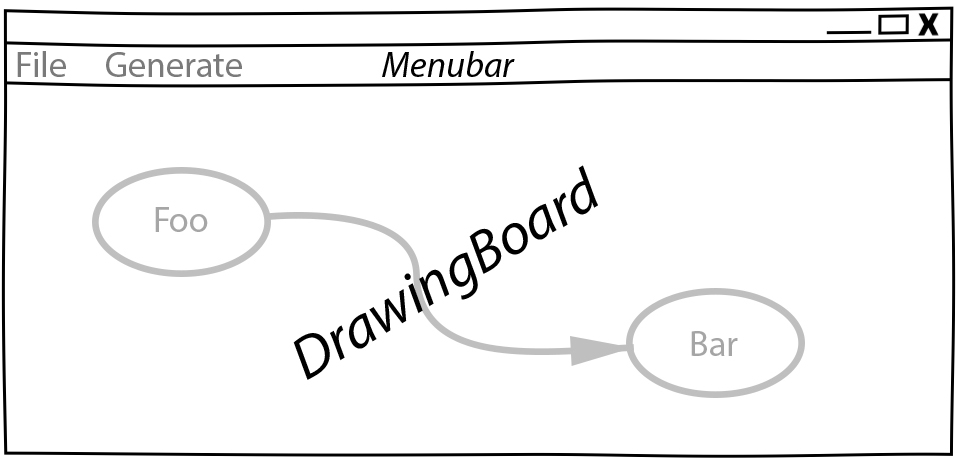
\includegraphics[width=.9\linewidth]{./img/MainCrop.jpg}
	\caption{Die Hauptansicht. Die Anwendung soll möglichst viel Platz für die Zeichenfläche
		bieten}
\end{figure}





\begin{figure}[H]
	\centering
	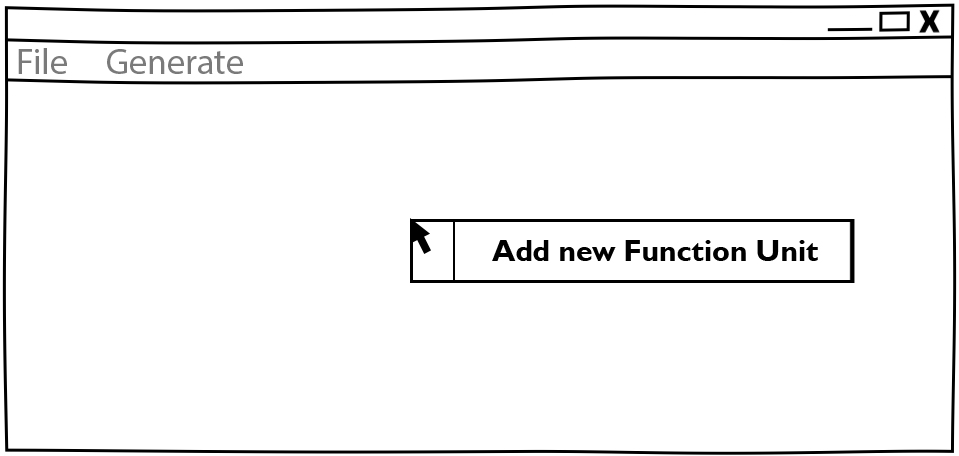
\includegraphics[width=.9\linewidth]{./img/ContextMenu.jpg}
	\caption{Bei einem Rechtsklick auf eine leere Stelle in der Zeichenfläche erscheint ein Kontextmenu, dass dem Anwender erlaubt an dieser Stelle eine neue Funktionseinheit einzufügen.}
\end{figure}


\begin{figure}[H]
	\centering
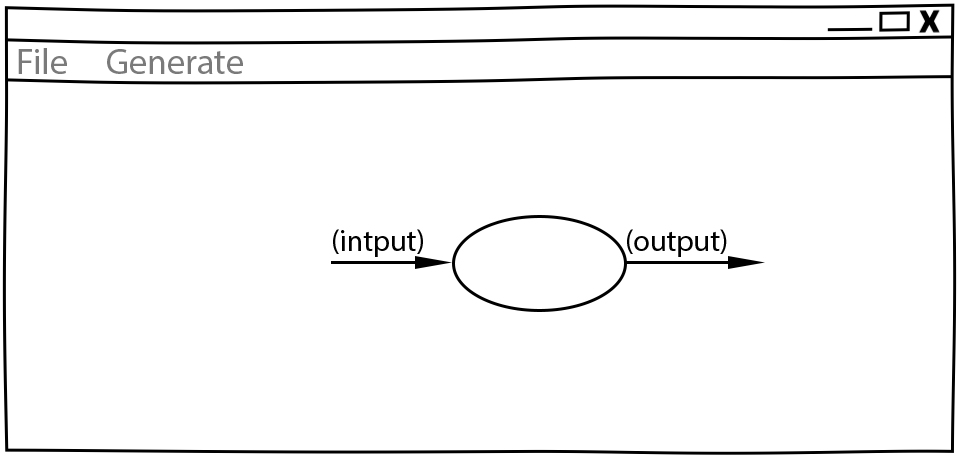
\includegraphics[width=.9\linewidth]{./img/NewCell.jpg}
	\caption{Eine neue Funktionseinheit wurde erstellt}
\end{figure}




\bigskip
Im folgendem einige Kerngedanken über die Funktionalität des Editors:

\begin{itemize}
\item Keine unnötigen Menüleisten, Symbolleisten, etc. Besser kontextsensitive
Kontextmenüs, oder Hotkeys,  damit die Strecke, die die Maus bewegt werden muss, gering
gehalten wird.
\item Tabulatorstopps einbauen, damit schnell zwischen den Textfeldern, entlang des
Graphen, gesprungen werden kann.
\item Verwendung von Drag\&Drop, um eine intuitive Bedienung zum Verknüpfen von
Funktionseinheiten zu ermöglichen. Die Flächen, die per Drag\&Drop zu Bedienen
sind, sollen über ein Mouse-Hover Feedback erkennbar sein. Außerdem sollen die
Flächen nicht zu klein sein, damit ein leichtes Treffen des Feldes
sichergestellt wird. Möglicherweise können auch unsichtbare Flächen verwendet
werden, um eine Drag\&Drop Fläche künstlich leicht zu vergrößern und einfacher treffbar zu machen.
\item Rectangle-Selection in Kombination mit Modifier-Keys um mehrere Funktionseinheiten
schnell und komfortable zu selektieren.
\item Shift + Drag : Schnelles Duplizieren der selektierten Elemente. 
\footnote{Vorbild dieser Funktion ist die CAD-Anwendung 3ds Max, das dieses Bedienkonzept an vielen Stellen einsetzt.
Einmal daran gewöhnt, möchte man es nicht mehr missen.} 

Anwendungsfälle:
Der Anwender möchte  schnell ein gesamtes Diagramm duplizieren und an ein andere Stelle schieben, um
dort eine weitere Iteration davon zu erstellen. Möglicherweise müssen solche
Duplikate vor der Generierung des Codes aus dem Diagramm gelöscht werden.
Ein andere Anwendungsfall von Duplizierten ist, dass der Anwender eine vorhandene
Funktionseinheit an einer anderen Stelle im Diagramm verwendet möchte. Damit
entstehen weitere Probleme, bei der Generierung des Codes, das gelöst werden
muss: Duplizierte Funktionseinheiten müssen erkannt und nur einmal generiert werden.
\item Ctrl + Drag einer Funktionseinheit: Die Funktionseinheit und alle ihre Kinder werden
Verschoben. Anwendungsfall ist: Der Anwender möchte etwas Platz schaffen
zwischen zwei Funktionseinheiten. Mit einem Ctrl+ Drag der zweiten Funktionseinheit,
kann er diese und alle nachkommenden Funktionseinheiten verschieben, ohne sie
vorher extra selektieren zu müssen.
\end{itemize}

\section{Textfelder}

Textfelder müssen waagerecht bleiben. Auf dem Papier schreibt man die Daten auf
die Pfeile, somit wird Text auf einem schrägen Pfeil auch entlang des Striches
geschrieben.
Am Computer ist so etwas schlecht umzusetzen. Man kann Textfelder bei WPF drehen, dadurch
entsteht jedoch eine ungewohnte Bedienung beim Markieren von Text. Ein Drehen
beim Fokussieren/Defokussieren wäre auch möglich, damit wäre jedoch eine zusätzlicher
Klick nötig, falls man Text markieren möchte: Ein Mausklick zum Fokussieren/Drehen
der Textbox und ein weiterer um Text zu markieren / den Cursor zu platzieren.
Die beste Lösung wäre aus Usability-Sicht, wenn Textfelder nicht gedreht werden,
sondern immer waagerecht dargestellt werden. Somit muss hier die Notation an
manchen Stellen etwas vom original Abweichen.
\begin{itemize}
\item Mehrere Outputs
\item Pfeile zwischen zwei Funktionseinheiten, die auf unterschiedlichen Höhen platziert
sind.
\end{itemize}

\emph{Mehrere Outputs}



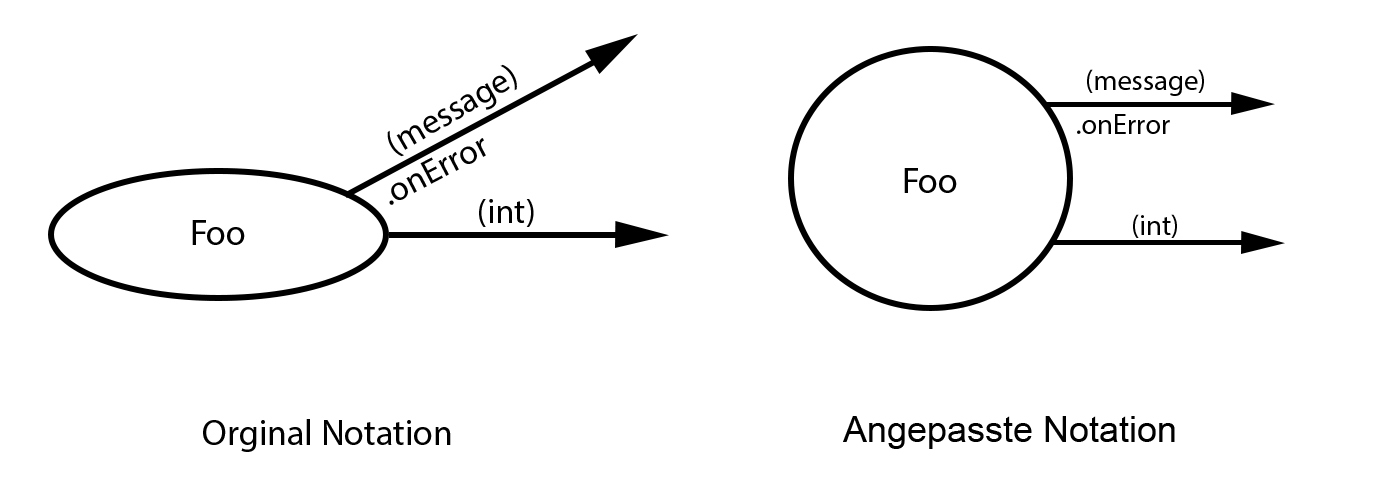
\includegraphics[width=.9\linewidth]{./img/NotationChanges1.jpg}
\bigskip

\emph{
Pfeile zwischen zwei Funktionseinheit, die auf unterschiedlichen Höhen platziert
sind}

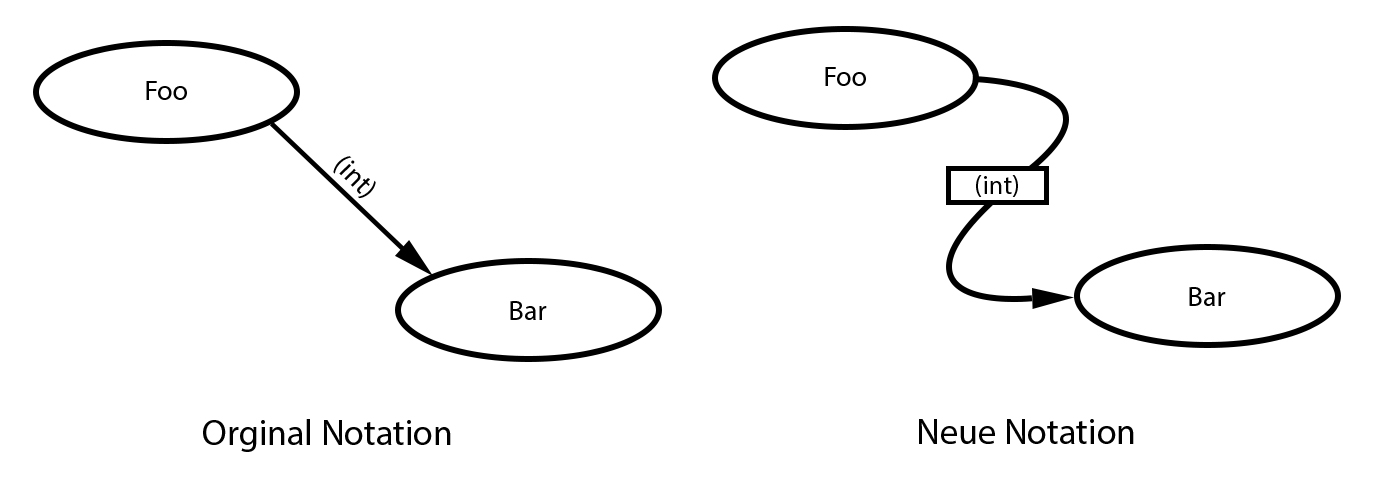
\includegraphics[width=.9\linewidth]{./img/NotationChanges2.jpg}



\section{Datentypen - Definition und Organisation}

Da Flow Design mit Datenströmen arbeitet, ist das Definieren neuer Datentypen
ein wesentlicher Bestandteil davon.
Eine Möglichkeit wäre es, wie auf dem Papier, es zu erlauben an beliebigen
Stellen im Diagramm eine Box zu erstellen, in der der Anwender einen neuen
Datentyp benennen und seine Felder definieren kann. Vorteil davon wäre, dass der
Anwender die nötige Information in der Nähe des Datenstroms schnell ersichtlich
platzieren kann, wo die Daten auch vorkommen.

Nachteil wäre, dass der Algorithmus zum automatischen Spacing komplizierter
werden würde, da nun auch eine sinnvolle Platzierung der Datentypen nun mit
berücksichtigen werden müsste.
Ein weiteres Problem dieser Lösung taucht auf, sobald der Anwender an unterschiedlichen
Positionen im Diagramm den selben Datentypen verwendet. In diesem Fall müssten Doppelungen erlaubt
sein, oder der Anwender würde an einer Stelle nicht die Information haben, worum
es sich bei einem Datentyp handelt.

Eine andere Option wäre es, die Datentypen nicht auf dem Drawing-Board zu
platzieren, sondern separate vom Flow Design getrennt in einem extra GUI-Element
darzustellen und dort die Definition eigener Datentypen zu ermöglichen.
Dieses GUI-Element würde in Form einer Liste alle vorhanden Datentypen
beinhalten. Zusätzliche Usability-Features wären, das Typen, die im Diagramm
vorkommen, jedoch nicht zu den Basistypen der Sprache gehören und noch nicht in
der Anwendung definiert wurden, erkannt und speziell hervorgehoben werden und
den Anwender subtil auffordert diesen zu definieren.

Um den Vorteil einer Box innerhalb des Diagrammes etwas zu entkräften, könnten
die Einträge in der Liste kontextsensitiv sein: Wenn der Anwender in ein
Textfeld eines Datenstromes klickt, könnte die Liste nur jene Datentypen
anzeigen, die in dem Textfeld vorhanden sind. Beim klick auf eine leere Fläche (
defokussieren des Textfeldes) würden wieder alle Datentypen im gesamten Diagramm
angezeigt werden. Desweiteren wäre eine visuelle Hervorhebung von nicht
verwendeten Datentypen auch denkbar.
\bigskip

\begin{figure}[H]
	\centering
	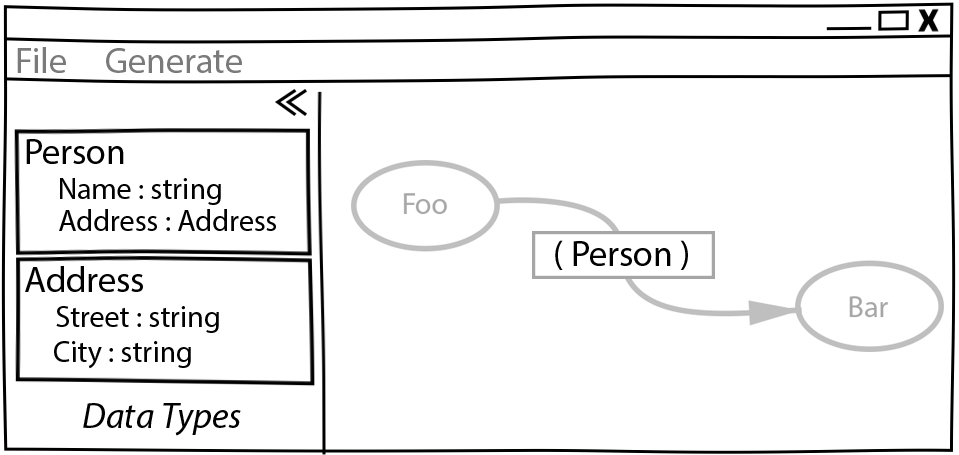
\includegraphics[width=.9\linewidth]{./img/DatatypesCrop.jpg}
	\caption{Datentypen Editor}
\end{figure}




Weitere Ideen: 
\begin{itemize}
\item Mouse-Hover über ein Datentype im Diagramm zeigt die Definition in einem Pop-Up
über dem Mauszeiger an.
\item Drag\&Drop von Datentypen aus der Liste in das \textit{DrawingBoard} zu
ermöglichen, falls der Anwender für einen Screenshot - oder aus einem anderen
Grund - diese Information im Bild haben möchte.
\end{itemize}


\section{Darstellung von Joined Inputs}

Datenströme können aus verschieden Quellen stammen und an einer Funktionseinheit
zusammenlaufen. Flow Design bietet hierfür die Pipe-Notation, oder die s.g. Joined Inputs an. 

\bigskip

Vorteile der Pipe-Notation:

\begin{itemize}
\item Einfacher zu realisieren auf GUI Seite ( Automatisches Spacing aufgrund der
geringeren Anzahl an Pfeilen einfacher umzusetzen
\item Pfeile müssen seltener große Distanzen überbrücken, was das Diagramm weniger
chaotisch wirken lässt
\end{itemize}

Nachteile der Pipe-Notation / Vorteile der Joined Inputs:

\begin{itemize}
\item Datenströme sind möglicherweise nicht mehr eindeutig zu interpretieren. 
Bei der Verwendung von Joined Inputs ist die Herkunft eines Datenstroms eindeutig
ersichtlich. Bei der Pipe-Notation kann man diese Problem durch eine Benennung der Daten auf den Datenströmen lösen. Diese Erkenntnis legt eine Validierung - einschließlich visuellem Feedback - der Datenströme auf eine eindeutige Interpretation nahe.
\end{itemize}

Da beide Notationen ihre Vor- und Nachteile haben, soll die Anwendung beide Darstellungen unterstützen.

\section{Validierung des Datenflusses}

Der Validierungsprozess soll subtil sein. Ein Blockieren beim Verbinden zweier Funktionseinheiten soll nicht geschehen. Diese würde sonst dem Ziel entgegen stehen,
eine möglichst freie Gestaltung, wie beim Zeichnen auf dem Papier, zu
gewährleisten. Der Anwender soll die Freiheit haben, nicht valide Verbindungen
zu erstellen, die er möglicherweise erst nach dem Verbinden dann entsprechend
anpasst. Eine dezente farbliche Hervorhebung soll als Feedback des
Validierungsprozesses ( möglicherweise indem man den Pfeil einfärbt) ausreichen. Mögliche Validierungsfehler wären:
\begin{itemize}
\item Pipe-Notation : Überschneidung von Datentypen.
\item Fehlende Daten : Nicht alle vom Input der Funktionseinheit verlangten Daten
sind im Datenfluss enthalten.
\end{itemize}

Im Grunde wäre jedoch auch eine Generierung von jeglichen Flow Design Diagrammen
möglich, würde man folgende Regeln einführen:

Der Graph wird zurück gelaufen, bis ein passender Datentype
gefunden wird (das erste Vorkommen wird genommen). Falls der Datentyp nicht
gefunden wird, wird er in der Integration als lokale Variable deklariert und mit einem Standardwert initialisiert.


\section{Validierung der Syntax}

Die Notation der Daten der Datenflüssen besteht aus einer einfachen Syntax. Diese muss zwingend eingehalten
 werden, damit eine Generierung des Codes möglich ist.
 Eine rote gewellte Linie unterhalb des nicht validen Textes soll dem Anwender
 anzeigen, dass ein Syntaxfehler vorhanden ist.


	


\chapter{Realisierung }

	\begin{figure}[H]
		\centering
		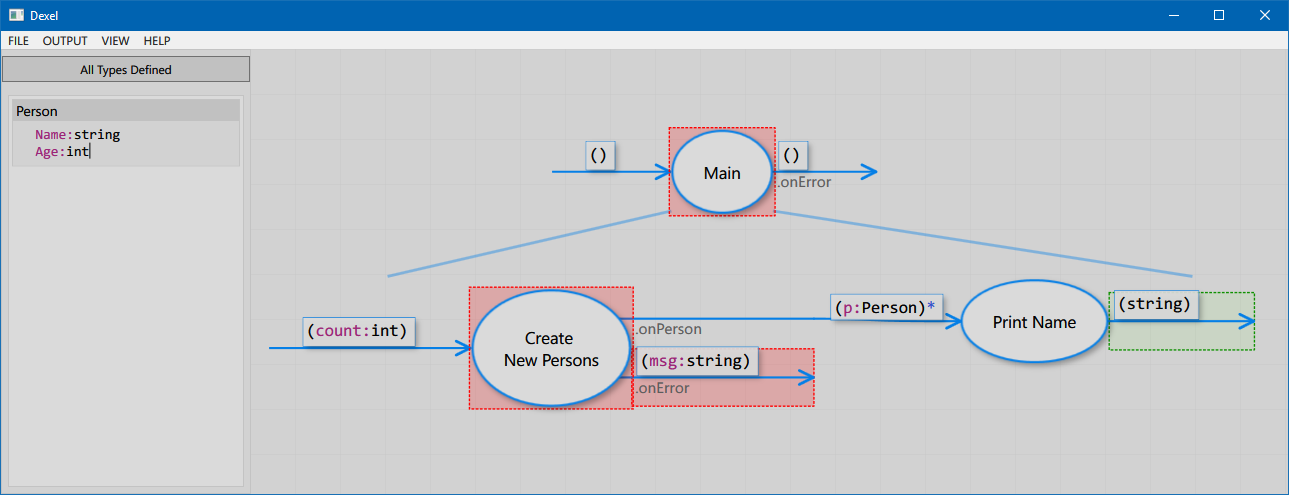
\includegraphics[width=1\linewidth]{./img/Dexel.png} 
		\caption{Dexel}
	\end{figure}



In diesem Kapitel soll vorgestellt werden, was in dem Zeitraum dieser
Bachelorarbeit erreicht wurde. Die Architekur der Anwendung wurde selbst nach
Flow Design umgesetzt und bietet somit dem Leser eine Quelle an weiteren
konkreten Beispielen aus der Praxis, wie eine Methode nach IOSP in der Praxis aussieht.

Als Arbeitstitel für die Anwendung wurde der Name Dexel gewählt.

\section{Übersicht über die unterschiedlichen Projekte}

Die Anwendung besteht aus einer \textit{Solution}, die folgende Unterprojekte beinhaltet \footnote{Bei komplexen Funktionalitäten wurde nach TDD (Test Driven Development)
programmiert, bei dem zuerst der Test geschrieben wird, der das zu erwartende
Ergebnis definiert, und erst anschließend die Methode implementiert wird.
. Diese Tests wurden in einem extra Test-Projekt für jedes Projekt zusammengefasst.}:

\subsubsection{Dexel.Model / Dexel.Model.Tests}

Dieses Projekt beinhaltet das Domänenmodell - alle Datentypen die zur internen Repräsentation
eines Flow Design Diagrammes nötig sind. Außerdem beinhaltet dieses Projekt
statische Manager-Klassen, die das Arbeiten mit den Datentypen vereinfachen.

\subsubsection{Dexel.Editor / Dexel.Editor.Tests}

Dies ist das Hauptprojekt, das alle anderen Projekte integriert.
Nach Flow Design kann man IOSP auf Projekt-Ebene anwenden, hier wurde jedoch das IOSP
Prinzip nicht eingehalten. Dieses Projekt hat nicht nur die Aufgabe die
anderen Projekte zu integrieren, sondern beinhaltet selbst den
UI-Sourcecode. Diese Entscheidung wurde gefällt, da ein Extrahieren der UI
in ein anderes Projekt sich als zu schwierig erwies. Eine Lösung dafür zu
finden, wie ein Event aus dem UI mit einer Funktionalität verbunden werden
könnte, dass sich in einem Projekt befindet, war zeitlich zu
aufwendig. Aus diesem Grund wurde entschieden auf die zusätzliche
Komplexität einer Entkoppelung zu verzichten und es einfacher zu halten, indem
dieses Projekt sowohl die UI beinhalter, als auch alle anderen Projekte
kennt.

\subsubsection{Roslyn / Rosyln.Tests}

Diese Projekt beinhaltet die Logik zur Erstellung von C\#-Code aus einem Flow
Design. Mircosoft Rosyln ist die Technik, die hier zum Erstellen von Code zum
Einsatz kommt.
Das Flow Design Diagramm muss in Form eines Mainmodels aus dem
Dexel.Model Projekt vorliegen. Aus diesem Grund gibt es eine Abhängigkeit
zwischen diesem Projekt und dem Dexel.Model Projekt. 

Eine Trennung dieser Abhängigkeit wurde versucht umzusetzen indem gegen ein Interface
programmiert wurde, anstatt gegen die konkrete Implementation in
Dexel.Model. Diese Interfaces der Datentypen und Manager-Klassen wurde dann
in ein Contracts-Projekt ausgelagert, von dem alle anderen Projekte abhängig
sein durften. Die zusätzliche Komplexität, Mehraufwand und ein Problem bei
der Serialisierung von Datentypen, die Interfaces als Eigenchaften besaßen,
machte es nicht wert hier eine Entkoppelung zu schaffen. Somit wurde der
Beschluss gefällt auf die Interfaces zu verzichten.

\subsubsection{Dexel.Library}

Dieses Projekt beinhaltet einige Methoden ( meist Extension-Methoden), die ein Arbeiten
nach Flow Design erleichtern. Diese wurden in ein separates Projekt
ausgelagert, damit alle anderen Projekte darauf zugreifen können.

\section{Das Domänenmodell}

Um nachfolgende Kapitel der Realisierung und die darin enthaltenden
Codeauschnitte verstehen zu können, braucht es ein Verständnis darüber, wie die
grundlegenden Datentypen des Domänenmodells aufgebaut sind. Um die Funktionalität der
jeweiligen Datentypen besser zu veranschaulichen, werden in diesem Kapitel
Bilder verwendet, welche die spätere Darstellung des Datentypen in der UI zeigen.

\subsubsection{MainModel}

Das MainModel ist, wie der Name schon sagt, das Haupt-Modell, das alle
anderen Modelle per Komposition beinhaltet. Somit kann einer Methode einfach eine Objektinstanz
eines MainModels übergeben werden und erhält dadurch alle Informationen über das aktuelle Flow Design Diagramm. 
Das \textit{MainModel} beinhaltet alle Funktonseinheiten, alle verbindende
Datenströme (\textit{Connections}) und alle benutzerdefinierten Datentypen (\textit{DataTypes}).

\begin{lstlisting}[caption=MainModel Klasse]
[ImplementPropertyChanged]
public class MainModel
{
	public List<FunctionUnit> FunctionUnits { get; set; }
	public List<DataStream> Connections { get;  set; }
	public List<CustomDataType> DataTypes { get; set; } 
}
\end{lstlisting}

\subsubsection{FunctionUnit}


\begin{lstlisting}[caption=FunctionUnit Klasse]
[ImplementPropertyChanged]
public class FunctionUnit
{
	public Guid ID { get; set; }
	public string Name { get; set; }
	public Point Position { get; set; }
	public List<FunctionUnit> IsIntegrating { get; set; }
	public List<DataStreamDefinition> InputStreams { get; set; }
	public List<DataStreamDefinition> OutputStreams { get; set; }
}
\end{lstlisting}

	
	\begin{figure}[H]
		\centering
		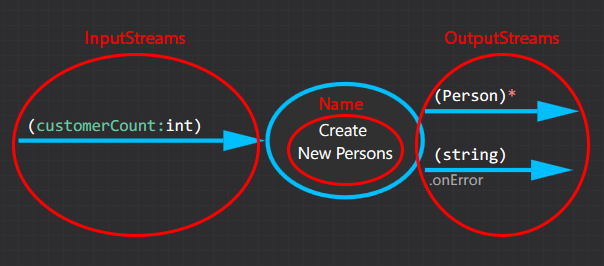
\includegraphics[width=0.9\linewidth]{./img/FunctionUnitView.png} 
		\caption{Dexel-Screenshot: FunctionUnit-View}
	\end{figure}

Der Name ist der Name der Funktionseinheit ( der Text, der bei der
Darstellung später innerhalb des Kreises erscheint). Dieser wird später per Binding
direkt an die UI gebunden. Aus diesem Grund implementiert dieses Klasse,
genau wie alle anderen des Modells, die ImplementPropertyChanged
Funktionalität. Diese bewirkt, dass bei einer Änderung im UI automatisch das
entsprechende Property im Modell aktualisiert wird und umgekehrt.

Die Position beschreibt die Position der Funktionseinheiten innherhalb des
Diagrammes.  

Das IsIntegrating Property gibt an, ob diese Funktionseinheit eine Integration
ist und welche andere Instanzen von Funktionseinheiten sie integriert.
Eine leere Liste besagt, dass die Funktionseinheit keine Integration ist.

Die Input- und OutputStreams definieren die möglichen ein- und ausgehenden
Datenströme der Funktionseinheiten. An diese DataStreamDefinitionen können sich DataStreams
verbinden. Dadurch lassen sie die Datenflüsse modellieren.


	\subsubsection{DataStreamDefinition}
	
	\begin{lstlisting}[caption=DataStreamDefinition Klasse]
[ImplementPropertyChanged]
public class DataStreamDefinition
{
	public Guid ID { get;  set; }
	public string DataNames { get;  set; }
	public string ActionName { get;  set; }
	public FunctionUnit Parent { get;  set; }
	public bool Connected { get;  set; }
}
	\end{lstlisting}
	
		
		\begin{figure}[H]
			\centering
			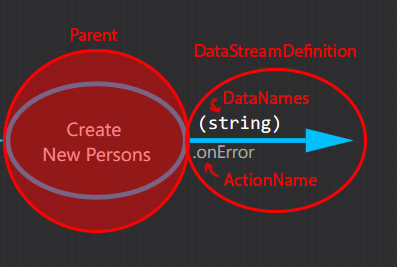
\includegraphics[width=0.6\linewidth]{./img/DataStreamDefinitionView.png} 
			\caption{Dexel-Screenshot: DataStreamDefinition-View}
		\end{figure}
	
	Eine Funktionseinheit verfügt über ein oder mehrere ein- und ausgehende
	DataStreamDefinitionen. Diese können verbunden sein oder nicht. Wenn eine
	Verbindung erstellt und gelöscht wird, muss deshalb auch das Connected
	Property immer gesetzt werden, damit das Model valide bleibt.
	Ob eine DataStreamDefinition verbunden ist, oder nicht, ist vorallem später
	für die Darstellung relevant.
	Eine DataStreamDefinition kennt auch die Funktionseinheit, von der sie ein
	Ein- oder Ausgang ist.
	
	Eine weitere grundlegende Eigenschaft ist die Benennung der Daten, die in/aus
	dem Ein-/ Ausgang fließen. Für Ausgänge ist auch die Angabe eines
	Actionnames manchmal nötig. Dieser soll später unterhalb des Pfeiles
	dargstellt werden.


\subsubsection{DataStream (Connections)}

Um Datenflüsse zwischen Funktionseinheitn zu beschreiben, bedarf es einer
Verbindungsklasse. Die DataStream-Klasse stellt diese Verbindungsklasse dar.


\begin{lstlisting}[caption=DataStream]
[ImplementPropertyChanged]
public class DataStream
{
	public Guid ID { get; set; }
	public string DataNames { get;  set; }
	public List<DataStreamDefinition> Sources { get;  set; }
	public List<DataStreamDefinition> Destinations { get;  set; }

}
\end{lstlisting}

		\begin{figure}[H]
			\centering
			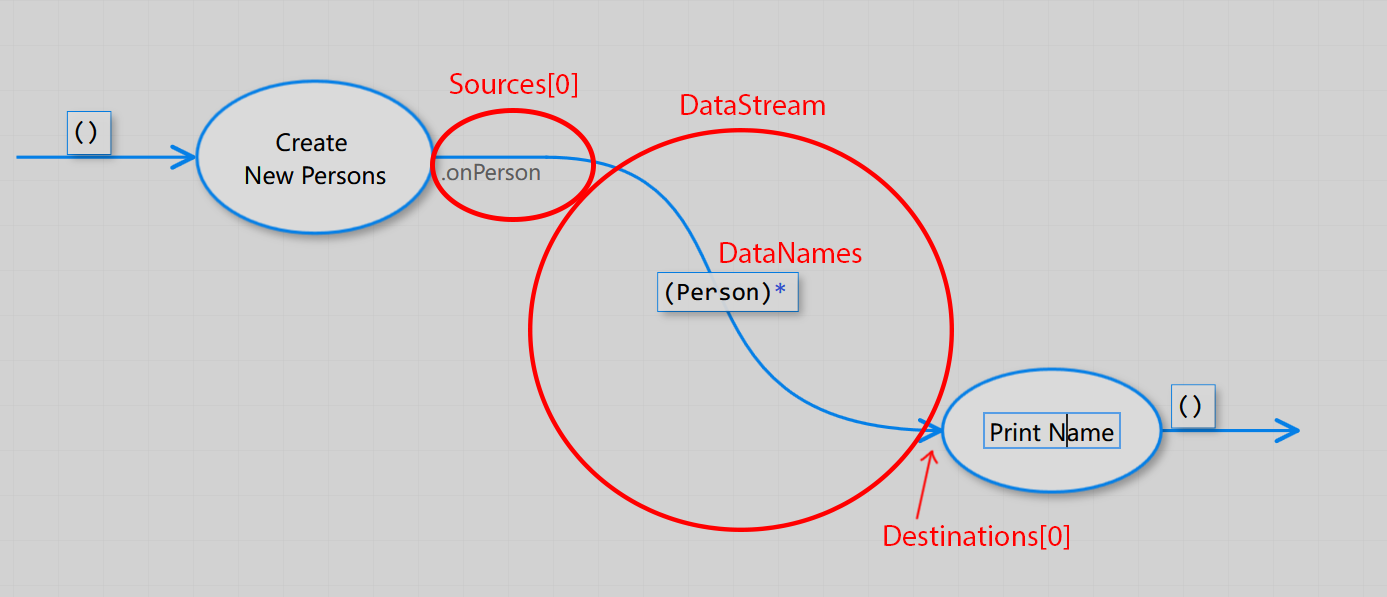
\includegraphics[width=0.9\linewidth]{./img/DataStreamView.png} 
			\caption{Dexel-Screenshot: DataStream-View}
		\end{figure}


Ein DataStream hat ein oder mehrere Referenzen an DataStreamDefinition als
Quellen und ein oder mehrere Referenzen an DataStreamDefinition als Ziele.
Um ein Datenstrom zu beschreiben, der aus mehren Quellen Daten bezieht und
an einer Stelle zusammenläuft, benötigt man ein DataStream, der mehrer
Einträge in der Source-Liste besitzt und ein Eintrag in der
Destination-Liste. Diese Datenstrom wäre dann ein Joint-Input.
Ein Datenstrom mit einer Quelle und mehreren Zielen wäre ein Joint-Output ( TODO:
Referenz auf vorheriges Kapitel)

Das DataNames Property stellt den Text dar, der später in der Mitte des
Pfeiles dargestellt werden soll. Eine Änderung dieser Eigenschaft bedarf
einer Aktualisierung der DataNames aller Sources und Destinations.
Eine Aktualisierung muss die optionalen Pipe-Notation kennen und
entsprechend dieser die Ein und Ausgänge akutalisieren.

Der akutelle Stand der UI kann akutell nur Datenflüsse mit einer Quelle und
einem Ziel darstellen.

\subsubsection{DataType}


\begin{lstlisting}[caption= CustomDataType und SubDataType Klasse]
[ImplementPropertyChanged]
public class CustomDataType
{
	public string Name { get; set; }
	public List<SubDataType> SubDataTypes { get; set; }
}

[ImplementPropertyChanged]
public class SubDataType
{
	public string Name { get; set; }
	public string Type { get; set; }
}
\end{lstlisting}


\begin{figure}[H]
	\centering
	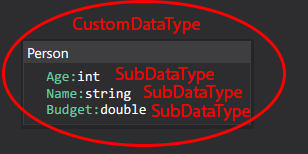
\includegraphics[width=0.5\linewidth]{./img/CustomDataType.png} 
	\caption{Dexel-Screenshot: CustomDataType-View}
\end{figure}


Ein benutzerdefinierter Datentyp besteht aus einem Namen und einer Liste von mehreren
\texttt{SubDataType}-Objekten. 

Ein SubDataType besteht aus einem Namen und den Namen
des Types (zum Beispiel string, int oder auch ein anderen benutzerdefinierten
Datentypen).

\subsubsection{Manager-Klassen}

\begin{enumerate}
	\item MainModelManager
	
	Einer der relevantesten Manager-Klassen ist die MainModelManager-Klasse,
	diese stellt die wichtigsten Funktionalitäten zur Verfügung die mit dem
	Arbeiten des MainModels gebraucht werden. Einige dieser Funktionalitäten
	wären: Verbinden und Trennen von Funktionseinheiten, vorwärts und rückwärts
	Traversieren entlang des Graphen, Hinzufügen und Entfernen einer
	Funktionseinheit von einer Integration, Hinzufügen, Löschen und Duplizieren
	von Funktionseinheiten, oder Teile des Graphen.
	
	\item DataStreamManager
	
	Diese statische Klasse bietet einige Funktionalitäten, die das Arbeiten mit
	Objekten der DataStream-Klasse vereinfachen soll.
	
	Ein Beispiel hierfür wäre das Ändern des Datanames eines DataStreams. 
	Wie bereits in letzten Abschnitt erwähnt, muss beim Ändern der Daten
	eines Datenflusses auch die Daten seiner Sources und Destinations
	angepasst werden. 
	
	Um dies nochmal zu verdeutlichen, zwei konkrete Beispiele:
	Falls der Datenfluss auf \textbf{(int) | (string) } geändert wurde
	, so muss die Source-DataStreamDefinition auf \textbf{(int)} gesetzt werden und der
	die Destination-DataStreamDefinition auf \textbf{(string)}. 
	Falls der Datenfluss auf \textbf{(double)} geändert wurde, so müssen Source-
	und Destination-Daten auf  \textbf{(double)}  gesetzt werden.\footnote{	Da aktuell nur DataStreams mit einer Source und einer Destination im Editor unterstützt
		
		werden, wurde akutell auch nur dieses Szenario implementiert. Ändert sich
		diese Einschränkung müsste man sich Gedanken darüber machen, was in diesen
		Fällen zu tun wäre. Ein Option wäre, die Pipe-Notation in diesen Fällen zu
		verbieten. Die UI würde die Daten der DataStreamDefinitionen direkt
		anzeigen und der Benutzer würde diese dann direkt ändern. Der Datenstrom
		selbst würde dann kein eigenes Textfeld besitzen und die Dataname
		Eigenschaft hätte in diesen Fall keine Bedeutung. 
		Vielleicht wäre es dann auch besser im Modell zwei separate Klassen
		anzulegen und die
		einfache DataStream-Klasse hätte anstatt einer Liste von DatastreamDefinitionen nur noch ein einfaches Feld
		für eine Source-DataStreamDefinition und eine Destionation-DataStreamDefinition.}
	
	\begin{lstlisting}[caption=ChangeDatanames Methode]
public static void ChangeDatanames(DataStream datastream, string newDatanames)
{
	// update datanames of connection itself
	datastream.DataNames = newDatanames;
	
	// update datanames of DSDs
	TrySolveWithPipeNotation(newDatanames,
		onSuccess: (outputPart, inputPart) =>
		{
			datastream.Sources.First().DataNames = outputPart;
			datastream.Destinations.First().DataNames = inputPart;
		},
		onNoSuccess: () =>
		{
			datastream.Sources.First().DataNames = newDatanames.Trim();
			datastream.Destinations.First().DataNames = newDatanames.Trim();
		});
}
\end{lstlisting}
	
\end{enumerate}



\section{Der Editor}

\subsection{Vorstellung was erreicht wurde}


Die Grundlegenden Basisfunktionen aus dem Anforderungs-Kaptitel wurden größtenteils implementiert. Hierbei kam WPF als GUI-Framework zum Einsatz.
Im folgendem einige Bilder und Beschreibungen der GUI und Interaktionen.


\subsubsection{	MISSING IMAGES Erstellen von Funktionseinheiten, Verschieben, Benennen, Selektieren}

	Das Drawing-Board wurde implementiert, auf dem der Benutzer mit einem
	Rechtsklick->Create New Function Unit eine erste Funktionseinheit erzeugen
	kann. Per Drag an Drop kann er diese dann innerhalb des DrawingBoards frei
	verschieben. Mit einer Rect-Selektion ist es mögliche mehrere
	Funktionseinheiten zu Selektieren. Selektierte Funktionseinheiten können
	gemeinsam verschoben, dupliziert und gelöscht werden.
	
	Nach dem Erstellen einer neuen Funktionseinheit, wird diese automatisch
	selektiert und der Tastaturfokus wird in das Textfeld des Kreises gesetzt.
	Durch lässt sich diese Benennen.
	
	Beim Klicken auf den äußeren Teil des Kreises wird die Funktionseinheit
	selektiert. Beim Klicken auf das Textfeld, wechselt der Tastaturfokus auf
	das Textfeld ( ein Mouse-Hover zeigt auch an, über welchen Teil des Kreises
	man sich gerade befindet, auch ein Klicken und Ziehen um sofort ein Teil
	des Textes zu markieren bleibt damit dem Benutzer möglich. Wie er es von
	einem Textfeld gewohnt ist).
	
	
\subsubsection{	 MISSING IMAGES Erstellen/Löschen/Manipulieren von Inputs und Outputs}

	Eine Funktionseinheit wird standardmässig mit einem Input und einem Output
	erstellt. Die Daten die aus diesen hinein- oder herausfließen können auf
	dem Textfeld eingetragen werden. Dabei bietet diese Textfeld ein einfaches
	Syntaxhighlighting, dass mit Doppelpunkt getrennte Namen-Type-Paare
	farblich trennt. Auch Symbole wie * | [] () , \ldots{} haben eine eigene Farbe.
	
	Der Action-Name kann unterhalb des Pfeiles eingetragen werden.
	
	Eine Funktionseinheit kann mehr als nur einen Output besitzen.
	Zum Hinfzufügen eines neuen Outputs: Rechtsklick -> Add New Output
	Das Löschen eines Outputs ist durch auch möglich: Rechtsklick auf ein
	Output -> Delete.    
	
	Die Reihenfolge bei mehreren Outputs kann per Drag and Drop verändert werden.
	
\subsubsection{MISSING IMAGES Verknüpfen und Trennen von Funktionseinheiten über Drag\&Drop }

	Wird das Ende eines Pfeiles eines Output auf ein Input Pfeil gedropt, so werden beide
	miteinandern Verbunden. Die Datennamen des Flusses werden bei nicht
	Übereinstimmung der beiden Daten des Input und Outputs mit
	der Pipe-Notation beschrieben. Stimmen beide Überein, kann darauf
	verzichtete werden.
	
	Werden die Daten eines verbundenen Datenflusses geändert, werden die Inputs
	und Outputs mit Berücksichtigung auf die Pipe-Notation angepasst, sodass
	beim Trennen der Beiden Funktionseinheiten, die Änderungen erhalten bleiben.
	
	Ein Drag \&Drop eines Outputs direkt auf eine Funktionseinheit: TODO
	
	Durch Drag and Drop eines verbunden Pfeiles auf eine leere Stelle auf dem
	DrawingBoard, kann eine Verbindung getrennt werden. Wird sie auf eine
	anderen Input gedropt, so wird diese als neues Ziel gesetzt und die 
	Verbindung zur vorherigen Funktionseinheit gelöscht. TODO
	
\subsubsection{	MISSING IMAGES Erstellen von Integrationen}

	Durch Rechtsklick auf eine Funktionseinheit kann im Kontextmenu der Eintrag
	'Make to Integration of (Pick)' ausgewählt werden. Der Cursor verändert
	sich und wird nun eine andere Funktionseinheit angeklickt, so wird der
	komplette Flow, in der diese Funktionseinheit Teil ist, als zu
	Sub-Flow der Integration genommen.
	
	Das Entfernen eines Flows von einer Integration geschieht indem auf eine
	Funktonseinheit rechtsklickt und dann auf 'Remove from Integration'
	ausgewählt wird. Der komplette zusammenhängede Flow wird dann aus der
	Integration entfernt. 
	
	
	Bei einer Modifikation des Datenflusses innerhalb einer Integration, werden nach
	bestimmten Regeln die nachfolgenden (abgetrennten) Funktionseinheiten
	ebenfalls aus der Integration entfernt. Wird die erste Funktionseinheit
	entfernt, gilt diese Regel nicht.
	
	\subsubsection{Definieren von Datentypen}

	Eigene DatenTypen können auf der rechten Seite des Editors angelegt werden.
	Durch Rechtsklick -> Add New DataType. Außerdem zeigt der obere Button an,
	ob im akutellen Diagramm Datenflüsse mit Daten fließen, die nicht definiert
	sind. ( int, string, double, usw. werden automatisch ignoriert). Ein Klick
	auf diesen erstellt für jeden nicht-definierten Datentyp ein neuen Eintrag.
	Auch Datentypen innerhalb eines eigenen Datentypen werden überprüft, ob sie 
	bekannt sind oder nicht. Bsp. 
	Person 
	name:string
	address:Address  
	
	Der Editor würde überprüfen ob der Address Datentyp definiert wurde oder nicht.
	
\subsubsection{MISSING IMAGES Navigation und Shortcuts}

	Zur Navigation innerhalb des DrawingBoards wird das Mausrad verwendet.
	Durch Scrollen wird in das DrawingBoard herein und herausgezoomt.
	Durch gedrückthalten des Mausrades (mittlere Maustaste) und Bewegen der
	Maus kann die Ansicht verschoben werden ( das DrawingBoard ist endlos groß)
	
	Ein weiteres Feature besteht darin, dass ab bestimmten Zoom-Stufen die
	Font-Größen der Namen der Funktionseinheiten angepasst werden und die 
	Textfelder der Datenflüsse ausgeblendet werden.
	Außerdem können Textfelder nicht mehr fokusiert werden, was ein einfachers
	Verschieben der Funktionseinheiten ermöglichen soll. Diese Eigenschaft wird
	visuell erkenntlich gemacht, dass die Hintergrundfarbe des Textfeldes bei
	einer selektierten Funktionseinheit nicht mehr dunkel ist.
	Auch der Mousecursor zeigt bei einem Mouse-Over an, dass man nicht mehr in
	das Textfeld klicken kann.
	
	
	\subsubsection{Weitere Features}

	\begin{itemize}
		\item Speichern, Laden, Mergen
		
		Das Speichern und Laden in 3 Dateiformate wird unterstüzt
		(yaml, json und xml - nach Dateigröße aufsteigend sortiert).
		Auch das Laden eines anderen Flow Designs in das aktuelle geladene wird 
		mit der Merge-Funktion unterstützt.

		\item Unhandled Exception ErrorDialog
		
		Wird eine Exception geworfen, die nicht behandelt wurde, so wurde eine
		allgemeine Fehlerbehandlung aufgerufen. Das Programm stürzt nicht ab,
		sondern ein Dialog errscheint, mit einem Stacktrace und Informationen
		über die geflogenen Exception. Der Benutzer kann das entscheiden, ob er
		hier das Programm Beenden will, oder weiter den Fehler ignorieren will.
		Der Stacktrace kann gegenenfalls kopiert und an den Entwickler als
		Bugreport zuschicken werden.
		
		\item Help-Window
		
		Ein simples Fenster gibt dem Benutzer einen Überblick über die
		vorhandenen Shortcuts und die Navigation mit der Maus wird erklärt.
	\end{itemize}
	



\subsection{Views / ViewModels}

Das Projekt wurde nicht strikt nach MVVM-Regeln (Model-View-ViewModel) 
umgesetzt, jedoch bedient es sich der Idee, das es eine View gibt, die
als Datenkontext ein ViewModel zugewiesen hat. Das Zuweisen eines
Datenkontextes erlaubt es GUI-Elemente der View an Propertys des ViewModels zu
binden. Ein Binding bewirkt, dass sich das GUI-Element automatisch aktualisiert,
sobald sich das dazugehörige Property ändert. Eine Änderung einer
Eigenschaft des ViewModels ändert somit automatisch die View.

Die GUI besteht aus mehreren Views (xaml-Dateien) und dazugehörigen ViewModels.
Die Aufgabe des ViewModels besteht vor allem darin, ein Model entgegenzunehmen und dieses
darzustellen, bzw. die aktuelle Darstellung zu aktualisieren.

Nach jeder Änderung am Model - zum Beispiel das Hinzufügen einer neuen
Funktionseinheit -  dieses komplett neu zu laden (Löschen und neu Hinzufügen aller
ViewModels, die wiederum ein neu Generieren der UI-Framework-Elemente zur
Folge hatte) erwies sich als nicht sehr performant. 
Ab Diagrammen, mit über 20 Nodes, stieg die Zeit zur Aktualisierung der View
bereits auf mehrere Sekunden an.
Die Lösung bestand darin, nicht einfach stur alles zu Löschen und neu
hinzuzufügen, sondern darin, die Änderungen am Model zu lokalisieren und nur
diese neu zu erstellen, bzw. nur die Propertys neu zu setzen. Durch
diese Verbesserungen wurde die Performance deutlich gesteigert, sodass
Diagramme mit mehreren hundert Funktionseinheiten keine spürbaren Perfomanceverluste mit
sich führt. Einzig das Duplizieren von vielen Funktionseinheiten dauert nach wie vor
mehrere Sekunden. 

\subsection{Interaktionen}

Wie bereits im Grundlagen-Teil erwähnt, (Abschnitt Entwurfsmethode) schlägt Flow Design
vor, alle Events als Interaktionen zu bezeichnen und für jedes dieser
Änderungen ein eigenen Flow Design zu erstellen. 
Es bietet sich somit an, alle Interaktionen in einer Klasse zu sammeln.
Diese bietet somit eine Überblick über alle Funktionalitäten der GUI.
Da diese Integrationen sind, sind sie leicht zu verstehen (mit Ausnahmen). Die
Interaktionen rufen Methoden von anderen Klassen auf, die die Operationen am
Mainmodel vereinfachen. Am Ende fast jeder Interaktion wird die \texttt{ViewRedraw}
Methode aufgerufen, die das \texttt{MainViewModel} veranlasst, das Model neu zu
laden und somit die Änderungen der Interaktion in der GUI sichtbar macht.
Deshalb erwies es sich als schlecht, wenn eine Interaktion eine andere
Interaktion aufruft, um ihre Funktionalität umzusetzen. 
Stattdessen war es eine bessere Lösung, den Code der einen Interaktion in
die andere zu Kopieren. Dies widerspricht zwar dem DRY Prinzip, jedoch eine
Coderedundanz innerhalb von Integrationen stellt sich als nicht sehr schlimm
heraus. Integrationen beinhalten schließlich keine Logik \footnote{Beim
Aufruf einer Funktionseinheit, die mehrere Outputs liefert, existiert
eigentlich doch Logik in der Integration ( Bsp: IsIntegration: Wenn ja,
dann X wenn nicht, dann Y). Dadurch verlieren Integrationen etwas an ihrer
Leichtgewichtigkeit und sind nicht mehr ganz so einfach zu verstehen} und haben eine hohe
Abstraktion.

Beispiel dieser Aussage:
\begin{lstlisting}[caption=AppendNewFunctionUnit]
public static object AppendNewFunctionUnit(FunctionUnit currentFunctionUnit, double offsetX, DataStreamDefinition outputToConnect, MainModel mainModel)
{
	var newFunctionUnit = FunctionUnitManager.CreateNew();
	
	newFunctionUnit.Position = currentFunctionUnit.Position;
	newFunctionUnit.MoveX(offsetX);
	
	// default IO of new function unit: input of new function unit = output to connect to of current function unit
	newFunctionUnit.InputStreams.Add(
		DataStreamManager.NewDefinition(newFunctionUnit, outputToConnect));
	newFunctionUnit.OutputStreams.Add(
		DataStreamManager.NewDefinition(newFunctionUnit, "()"));
	MainModelManager.ConnectTwoDefintions(outputToConnect, newFunctionUnit.InputStreams.First(), mainModel);
	
	mainModel.FunctionUnits.Add(newFunctionUnit);
	
	ViewRedraw();
	
	return newFunctionUnit;
}
\end{lstlisting}

\begin{lstlisting}[caption=CreateNewOrGetFirstIntegrated]
public static FunctionUnit CreateNewOrGetFirstIntegrated(FunctionUnit currentFunctionUnit, MainModel mainModel)
{
	FunctionUnit @return = null;
	
	currentFunctionUnit.IsIntegration(
		isIntegration: () => @return = 		currentFunctionUnit.IsIntegrating.First(),
		isNotIntegration: () =>
		{
			var newFunctionUnit = FunctionUnitManager.CreateNew();
			newFunctionUnit.Position = currentFunctionUnit.Position;
			newFunctionUnit.MoveY(100);
			
			newFunctionUnit.InputStreams.Add(
			DataStreamManager.NewDefinition(newFunctionUnit, currentFunctionUnit.InputStreams.First()));
			newFunctionUnit.OutputStreams.Add(
			DataStreamManager.NewDefinition(newFunctionUnit, "()"));
			
			currentFunctionUnit.IsIntegrating.Add(newFunctionUnit);
			
			mainModel.FunctionUnits.Add(newFunctionUnit);
			
			@return = newFunctionUnit;
			ViewRedraw();
		});
	
	return @return;
}
	\end{lstlisting}





	Die \texttt{AppendNewCell} Methode erzeugt eine neue Funktionseinheit und und
	verschiebt diese entlang der X Postion.
	Außerdem setzt sie den Input gleich der DataStreamDefinition die
	übergebenen wurde und verbindet diese beiden.
	\texttt{AppendNewCell} wird durch die Tastenkombination Ctrl-Tab ausgelöst, wenn
	sich der Tastaturfokus innerhalb eines Textfeldes einer View einer Funktionseinheit oder
	DatastreamDefinition befindet. Bei ersterem wird der erste unverbunden Output als der
	DataStreamDefinition genommen, an dem die neue Funktionseinheit angehängt wird \footnote{nicht Teil der gezeigten Methode} .
	
	Beide Methoden geben eine
	Model-Instanz als \texttt{object} an die GUI zurück. Die GUI-Logik findet dann die
	dazugehörige View und setzt den Fokus auf diese.
	
	Beide Methoden sind Methoden aus der Interaktions-Klasse, sind werden also
	direkt aus einem Event von der GUI ausgelöst. 
	Beide Methoden haben ähnliche Methodenaufrufe ( Neue Funktionseinheit
	erzeugen, sie auf die gleiche Position zu setzten wie die der übergebenen
	Funktionseinheit, neue Default-Werte für den Output-Stream der neuen
	Funktionseinheit setzen, dem MainModel die neue Funktionseinheit zu geben
	und die Ansicht neu zu zeichnen). Diese könnten in eine neue
	Integration ausgelagert werden, hätte jedoch eine unnötige
	Verschachtelung von Code als Auswirkung. Besser ist es hier die
	Coderedundanz als etwas nicht schlimmes anzusehen und diese zu belassen.
	So ist auf einen Blick ersichtlich, was die Interaktion genau macht, ohne
	im Code herumspringen zu müssen.

\subsection{Eigene Tabstop-Logik}

Mit Tab und Shift-Tab soll es dem Nutzer möglich sein den Tastaturfokus zu
verändern\footnote{Dieses Beispiel zeigt dabei noch einmal, das Coderedundanzen innerhalb
von mehreren Integrationen nichts Schlechtes sein muss.
Außerdem macht es auch deutlich, wie eine etwas komplexerer Integration mit
mehreren verschachtelten Lambda-Ausdrücken in der Praxis aussehen kann. Auch das Arbeiten mit dem \textit{Model} und den Managerklassen soll dem Leser hier noch einmal verdeutlicht werden.}.



Der nächsten Tabstop soll nach folgenden Regeln und abhängig vom aktuell
fokussierten \textit{Model} bestimmt werden:

\begin{enumerate}
	\item FunctionUnit

	Besitzt akutell die View einer FunctionUnit den Tastaturfokus, so soll als
	nächster Tabstop der erste Datenfluss, der verbunden ist gewählt werden. Ist keiner
	verbunden, wähle als nächsten Tabstop den ersten Output.
	
	\begin{figure}[H]
		\centering
		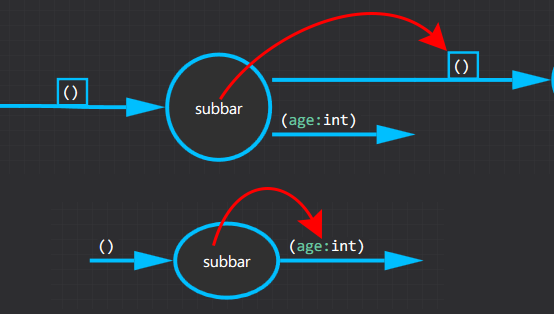
\includegraphics[width=0.6\linewidth]{./img/tabstop_functionunit.png}
		\caption{Aufgabe - Tabstop von FunctionUnit aus}
	\end{figure}
	
	\item DataStream

	 Wenn der Fokus aktuell auf einem DataStream liegt, so ist der nächste Tabstop die Ziel-Funktionseinheit des Datenflusses.

	\begin{figure}[H]
		\centering
		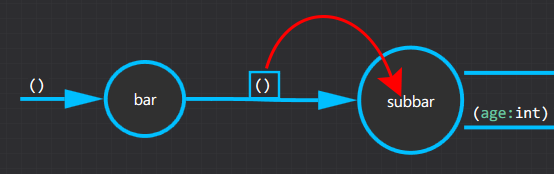
\includegraphics[width=0.6\linewidth]{./img/tabstop_datastream.png}
		\caption{Aufgabe - Tabstop von DataStream aus}
	\end{figure}
	
	\item DataStreamDefinition

	Der komplexeste Fall: 
	Zu erst muss überprüft werden, ob es sich um ein Input oder Output
	handelt. Ist es ein Input (A), so soll als nächster Stop die Funktionseinheit
	zurückgegeben werden, von der die DataStreamDefinition der Input ist. 
	Bei einem Output muss überprüft werden, ob das Ende des Flows erreicht
	wurde, oder nicht. Wird ein verbundener Output entdeckt, wird der
	entsprechende DataStream als nächster Stop zurückgegeben (B). Ist das Ende
	erreicht, so soll zum Anfang des kompletten Flows gesprungen werden (C).
	
	
	\begin{figure}[H]
		\centering
		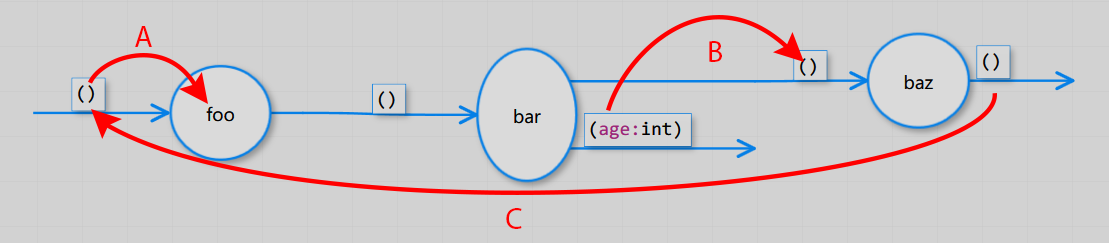
\includegraphics[width=\linewidth]{./img/tabstop_datastreamdefiniton.png}
		\caption{Aufgabe - Tabstop von DataStreamDefinition aus}
	\end{figure}
	
	\begin{lstlisting}[caption=Tabstop vorwärts]
public static object TabStopGetNext(object focusedModel, MainModel mainModel)
{
	object @return = null;
	
	focusedModel.TryCast<FunctionUnit>(fu =>
	{
		// prefer connected outputs as next tabstop
		// if no connected take first output defintion if there are any
		fu.OutputStreams.GetFirstConnected(
			foundConnected: connectedDsd => 
				@return =MainModelManager.FindDataStream(
				connectedDsd, mainModel),
			noConnected: () => 
				@return = fu.OutputStreams.FirstOrDefault());
		});
		
		focusedModel.TryCast<DataStream>(stream =>
		{
			// if focus was inside datastream take its destination function unit as next tabstop
			if (stream.Destinations.Any())
				@return = stream.Destinations.First().Parent;
		});
		
		focusedModel.TryCast<DataStreamDefinition>(dsd =>
		{
			// if focus was inside definition there are two case:
			// is input definition: next tabstop is the function unit of the definition
			// is output definition: in case the end of the flow was reached ( no connected output ) 
			// the next tabstop is the first input definition of the beginning of the whole flow.
			// Is the end not reached go to first connected output datastream
			dsd.CheckIsInputOrOutput( 
				isInput: () => @return = dsd.Parent,
				isOutput: () =>
			{
				dsd.Parent.OutputStreams.GetFirstConnected(
					foundConnected: connectedInput => 
						@return = MainModelManager.FindDataStream(
						connectedInput, mainModel),
					noConnected: () =>
					 // loop tabstop focus when the 
					 // end is reached
						@return = MainModelManager.GetBeginningOfFlow(
							dsd.Parent, mainModel)); 
			});
	});
	return @return;
}

\end{lstlisting}
	Analog dazu die Tabstop-Methode in die entgegengesetzte Richtung.
	
	
\begin{lstlisting}[caption=Tabstop rückwärts]
public static object TabStopGetPrevious(object focusedModel, MainModel mainModel)
{
	object @return = null;
	
	focusedModel.TryCast<FunctionUnit>(fu => 
	{
		fu.InputStreams.GetFirstConnected(
			foundConnected: connectedDsd => 
				@return = MainModelManager.FindDataStream(
				connectedDsd, mainModel),
		noConnected: () =>
			@return = fu.InputStreams.FirstOrDefault());
	});
	
	focusedModel.TryCast<DataStream>(stream => 
	{
		if (stream.Sources.Any())
			@return = stream.Sources.First().Parent;
	});
	
	focusedModel.TryCast<DataStreamDefinition>(dsd => 
	{
		dsd.CheckIsInputOrOutput(
			isOutput: () => @return = dsd.Parent,
			isInput: () => 
			{
				dsd.Parent.InputStreams.GetFirstConnected(
					foundConnected: connectedInput =>
						@return = MainModelManager.FindDataStream(
						connectedInput, mainModel),
					noConnected: () =>
						// loop tabstop focus when
						// the beginning is reached
						@return = MainModelManager.GetEndOfFlow(
						dsd.Parent, mainModel));
		});
	});	
	return @return;
}
\end{lstlisting}
	
	

	Auf oberster Ebene wird überprüft um welchen Typ von Objekt es sich
	handelt, der aktuell fokusiert ist \footnote{Teile davon war Aufgabe der UI und die
	Interaktion bekommt das Model dann als \texttt{object} übergeben. Deshalb bedarf es
	innerhalb der Methode einer Überprüfung des Typen mit TryCast.}. Nun existieren die drei Fälle, abhängig vom übergebenen Typen.\footnote{Zur Erinnerung: Die \texttt{Sources}-Eigenschaft eines \texttt{DataStream} beinhaltet nicht die Funktionseinheit,
	sondern die \texttt{DataStreamDefinition} einer Funktionseinheit. Die eigentliche
	Funktionseinheit enthält die \texttt{Parent}-Eigenschaft der \texttt{DataStreamDefinition}.
	Analog dazu enthält die \texttt{InputStream}- und \texttt{OutputStream}-Eigenschaft der
	Funktionseinheit auch nur die \texttt{DataStreamDefinition}-Objekte nicht ein \texttt{DataStream}-Objekt.
	Eine \texttt{DataStreamDefinition} kennt jedoch nicht den Datenfluss, mit dem sie
	verbunden ist. Eine Helfer-Methode der \texttt{MainModelManager}-Klasse stellt
	diese Funktionalität zum Auffinden des \texttt{DataStream} zur Verfügung.}
\end{enumerate}

\subsection{Validierung des Datenflusses - Farbliche Kennzeichnung }

Eigne ValidationException Klasse, die dem ViewModel übergeben werden kann. .
Die ValidationException beinhaltet die Information, ob es sich um eine Error oder um eine Warning handelt (Error wird rot markiert, Warnings grün), welche  Element den Fehler anzeigen sollen, und einen Fehlertext, der als Tooltip an dem Element abgezeigt wird.

\begin{figure}[H]
	\centering
	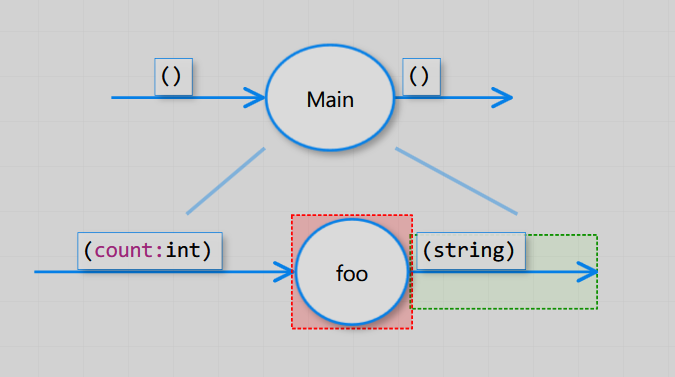
\includegraphics[width=0.6\linewidth]{./img/DexelValidation.png}
	\caption{Dexel - Warning- und Error-Darstellung}
\end{figure}



\section{Roslyn - Generierung von Code aus einem Diagramm}

Da eine Flow Design auf unterschiedlichen Weisen im Code umgesetzt werden
kann, mussten hier Entscheidungen getroffen werden, in welchen Fällen
welche Weise gewählt wird. Wird das Projekt weitergeführt, könnte man in
Betracht ziehen, dem Nutzer einige Optionen zur Konfiguration der Generierung
zur Verfügung zu stellen. Aktuell muss er sich jedoch damit abfinden, dass nur die hier vorgestellte Weise zur Verfügung steht.


\subsection{Vorstellung - was erreicht wurde}

Um den aktuellen Stand der Code-Generierung zu präsentieren, werden nachfolgend zwei Beispiele 
vorgestellt.

\subsubsection{CSV Tabellieren -  Beispiel aus YouTube Video von Ralf Westphal und Stefan Lieser}

Die Aufgabe besteht darin, den Inhalt einer CSV-Datei in eine ACSII-Tabelle zu formattieren.
\footcite[S.12]{kata}
\begin{figure}[H]
	\centering
	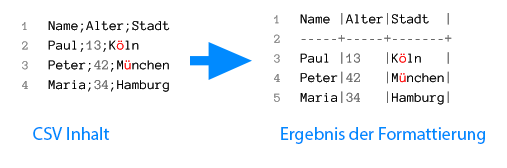
\includegraphics[width=0.8\linewidth]{./img/csvAufgabe.png}
	\caption{Aufgabe - CSV Tabellieren}
\end{figure}


Das Flow Design, das Ralf Westphal und Stefan Lieser in dem Video entwerfen sieht folgendermaßen aus. \footnote{Video CSV-Tabellieren \cite{youtubevideos}}


\begin{figure}[H]
	\centering
	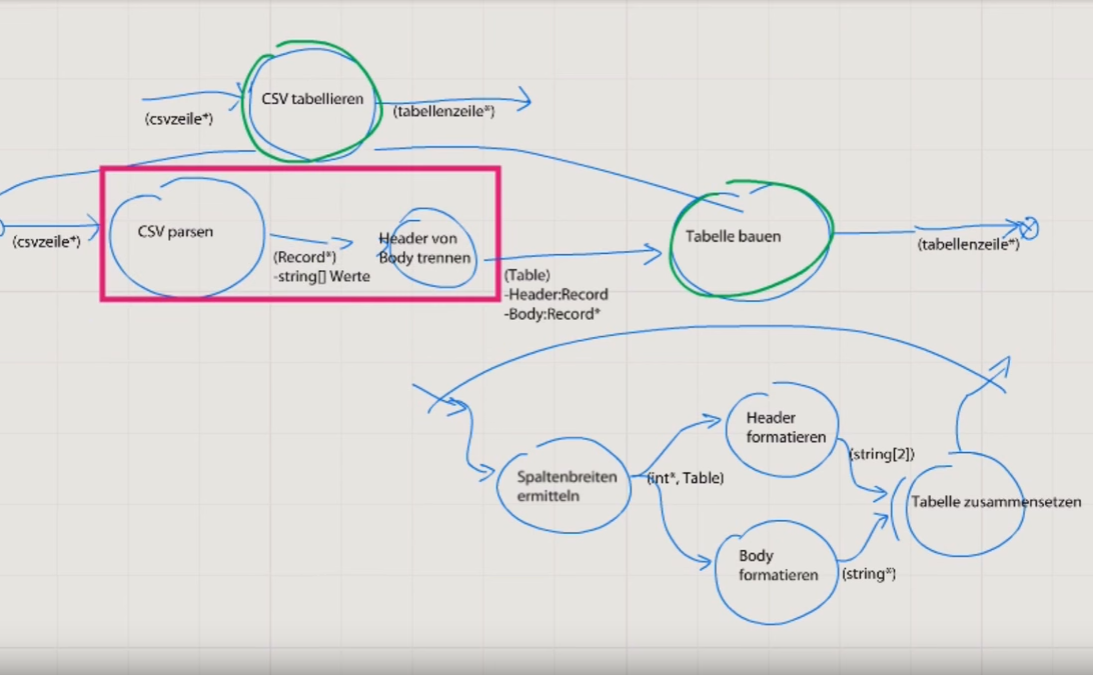
\includegraphics[width=1\linewidth]{./img/youtubeflowdesign.png}
	\caption{CSV Tabellieren - Flow Design aus YouTube Video}
\end{figure}


Nun das Flow Design umgesetzt in Dexel. Zu beachten ist, das die Joined Output und Joined Input Notation mit der Pipe-Notation ersetzt wurde, da Dexel akutell keine Joined-Notation unterstützt.


\begin{figure}[H]
	\centering
	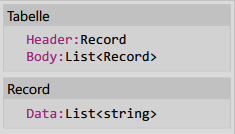
\includegraphics[width=0.4\linewidth]{./img/csvtabellierenDexelDataTypes.png}
	\caption{CSV Tabellieren - Flow Design aus YouTube Video}
\end{figure}




\begin{figure}[H]
	\makebox[\textwidth][c]{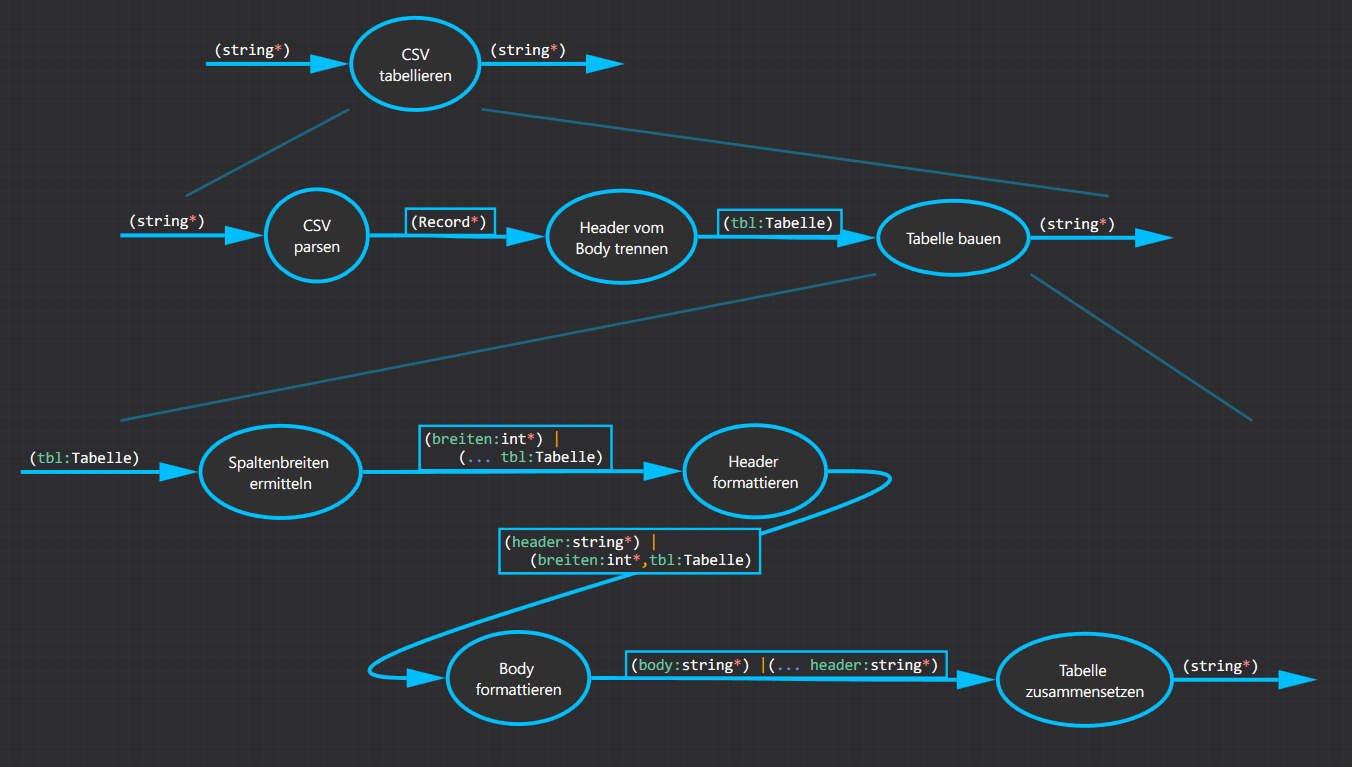
\includegraphics[width=1.2\textwidth]{./img/csvtabellierenDexel.png}}%
	\caption{CSV Tabellieren - Flow Design aus YouTube Video}
\end{figure}






\begin{lstlisting} [caption = CSV tabellieren mit Dexel generierter Code]

// Datentypen

public class Tabelle
{
    public Record Header;
    public List<Record> Body;
}

public class Record
{
    public List<string> Data;
}

// Integrationen

public static IEnumerable<string> CSVTabellieren( IEnumerable<string> strings)
{
	var records = CSVParsen(strings);
	var tbl = HeaderVomBodyTrennen(records);
	return TabelleBauen(tbl);
}

public static IEnumerable<string> TabelleBauen(Tabelle tbl)
{
	var breiten = SpaltenbreitenErmitteln(tbl);
	var header = HeaderFormattieren(breiten, tbl);
	var body = BodyFormattieren(breiten, tbl);
	return TabelleZusammensetzen(body, header);
}

// Operationen

public static IEnumerable<int> SpaltenbreitenErmitteln(Tabelle tbl)
{
    throw new NotImplementedException();
}

public static IEnumerable<string> HeaderFormattieren(IEnumerable<int> breiten, Tabelle tbl)
{
    throw new NotImplementedException();
}

public static IEnumerable<string> BodyFormattieren(IEnumerable<int> breiten, Tabelle tbl)
{
    throw new NotImplementedException();
}

public static IEnumerable<string> TabelleZusammensetzen(IEnumerable<string> body, IEnumerable<string> header)
{
    throw new NotImplementedException();
}

public static Tabelle HeaderVomBodyTrennen(IEnumerable<Record> records)
{
    throw new NotImplementedException();
}

public static IEnumerable<Record> CSVParsen(IEnumerable<string> strings)
{
    throw new NotImplementedException();
}


\end{lstlisting}

\subsubsection{Shopping Simulator - Komplexeres Beispiel}


\begin{figure}[H]
	\makebox[\textwidth][c]{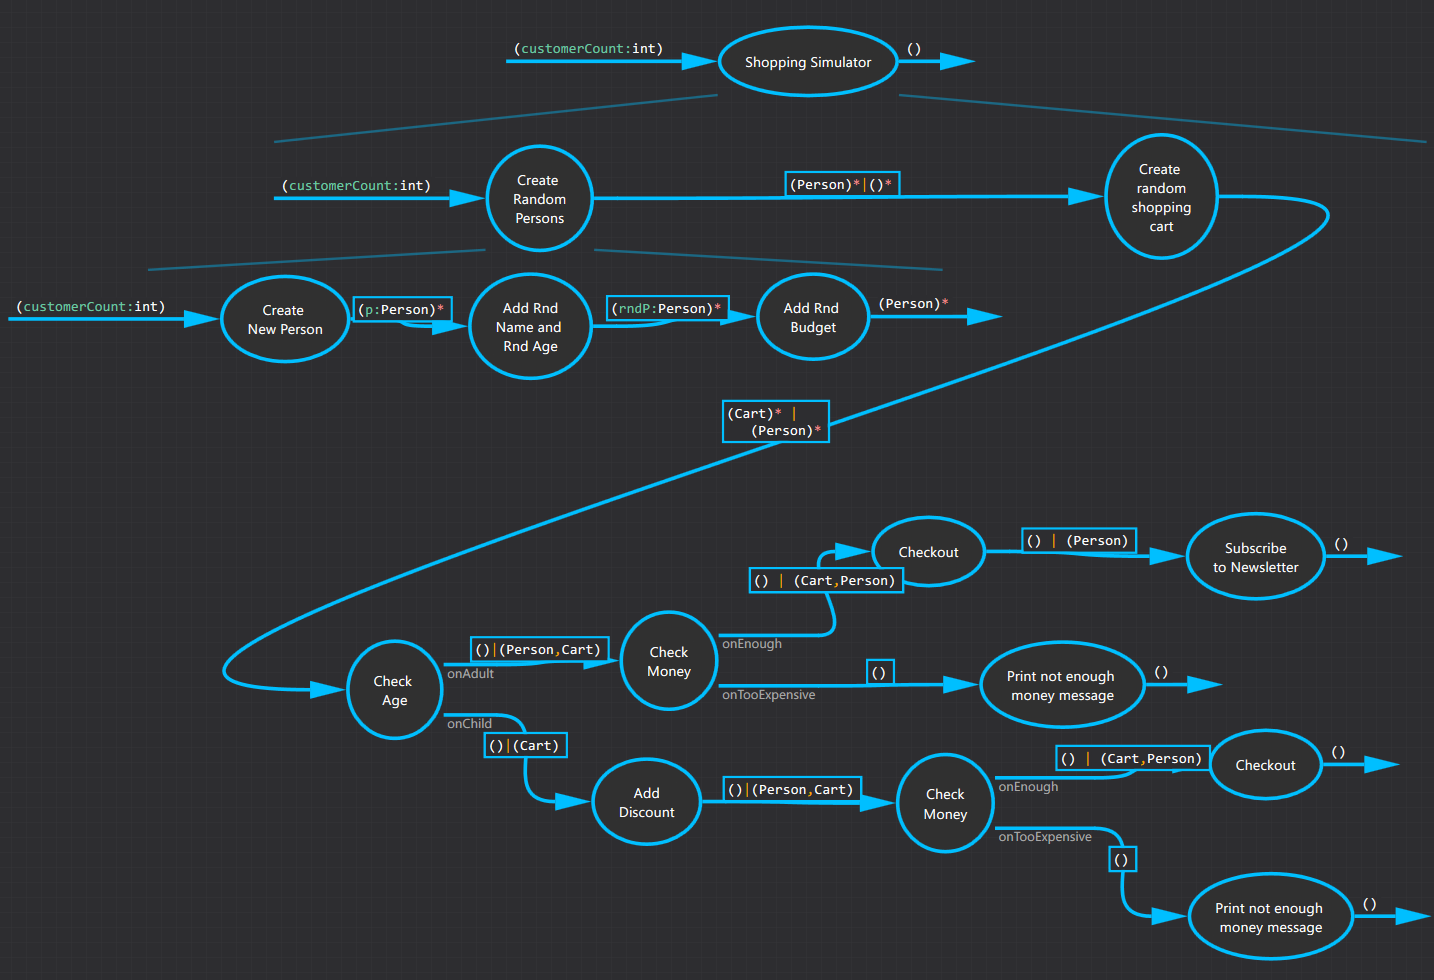
\includegraphics[width=1.2\textwidth]{./img/shoppingSimulator.png}}%
	\caption{Shopping Simulator}
\end{figure}


\begin{lstlisting}[caption=Shopping Simulator - automatisch generierter Code mit Dexel]

// Datentypen

public class Person
{
    public int Age;
    public string Name;
    public double Budget;
}

public class Cart
{
    public List<string> Products;
    public double Discount;
    public double PriceTotal;
}

// Integration

public static void ShoppingSimulator(int customerCount)
{
	CreateRandomPersons(customerCount, person => {
		var aCart = CreateRandomShoppingCart();
		CheckAge(person, onAdult: () => {
			CheckMoney(person, aCart, onEnough: () => {
				Checkout(aCart, person);
				SubscribeToNewsletter(person);
			}, onTooExpensive: () => {
				PrintNotEnoughMoneyMessage();
			});
		}, onChild: () => {
			AddDiscount(aCart);
			CheckMoney(person, aCart, onEnough: () => {
				Checkout(aCart, person);
			}, onTooExpensive: () => {
				PrintNotEnoughMoneyMessage();
			});
		});
	});
}

// Operationen

public static void CreateRandomPersons(int customerCount, Action<Person> onPerson)
{
	CreateNewPerson(customerCount, p => {
		var rndP = AddRndNameAndRndAge(p);
		onPerson(AddRndBudget(rndP));
	});
}

public static Cart CreateRandomShoppingCart()
{
    throw new NotImplementedException();
}

public static void CheckAge(Person aPerson, Action onAdult, Action onChild)
{
    throw new NotImplementedException();
}

public static void CheckMoney(Person aPerson, Cart aCart, Action onEnough, Action onTooExpensive)
{
    throw new NotImplementedException();
}

public static void AddDiscount(Cart aCart)
{
    throw new NotImplementedException();
}

public static void Checkout(Cart aCart, Person aPerson)
{
    throw new NotImplementedException();
}

public static void SubscribeToNewsletter(Person aPerson)
{
    throw new NotImplementedException();
}

public static void CheckMoney(Person aPerson, Cart aCart, Action onEnough, Action onTooExpensive)
{
    throw new NotImplementedException();
}

public static void PrintNotEnoughMoneyMessage()
{
    throw new NotImplementedException();
}

public static void PrintNotEnoughMoneyMessage()
{
    throw new NotImplementedException();
}

public static void Checkout(Cart aCart, Person aPerson)
{
    throw new NotImplementedException();
}

public static void CreateNewPerson(int customerCount, Action<Person> onP)
{
    throw new NotImplementedException();
}

public static Person AddRndNameAndRndAge(Person p)
{
    throw new NotImplementedException();
}

public static Person AddRndBudget(Person rndP)
{
    throw new NotImplementedException();
}


\end{lstlisting}

\subsubsection{Aktueller Stand}

Die weniger komplexeren Aufgaben wurden vollständig implementiert.
Diese wären: 
\begin{itemize}
	\item Generierung der benutzerdefinierten Datentypen, und 
	\item Generierung der Methodensignaturen einer Funktionseinheit.
\end{itemize}

Die weitaus komplexere Aufgabe: die Generierung der Methoden-Bodys einer Integration wurde nicht ganz vollständig implementiert.
Das liegt vor allem daran, dass eine vollständige Umsetzung einiges an manuellem Testen erfordert, um herauszufinden, welche Datenströme noch falsch interpretiert werden. 

Die Validierung des Datenflusses ist eng an die Generierung gekoppelt und deswegen gilt das selbe auch für diese. 

Auch bei der Generierung von Namen wird aktuell noch nicht in jedem Fall überprüft, ob es zu einer Überschneidung kommt und ob gegebenenfalls der Name angepasst werden muss.

\bigskip

Um Code zu generieren muss im Editor in der Menüleiste der Eintrag Output angesteuert werden.
Hier gibt es die Möglichkeit das aktuelle Flow Design in eine Datei auf den Desktop zu
generieren, den Code in die Konsole auszugeben, oder aber den Code direkt in die Zwischenablage zu kopieren( um den erzeugten Code bequem an eine gewünschte Stelle eingefügt werden kann).

Außerdem gibt es die Option eine automatische Generierung einzuschalten, die
den Code während der Bearbeitung immer neu generiert und in die Datei
auf den Desktop schreibt. So lässt sich das Ergebnis der Generierung während der Bearbeitung
des Datenflusses beobachten (vor allem in Kombination mit einem
Texteditor, wie zum Beispiel Atom, die bei einer Änderung der Datei diese automatische neu laden).

Das Ergebnis wird auch immer mit in die Konsole ausgegeben, die beim
Programmstart mit geöffnet wird.


\subsection{Kleiner Einblick in die API von Roslyn}

Das Projekt Rosyln von Microsoft ist ein .NET-Compiler, der eine API bietet, um beliebigen C\#-Quelltext zu erstellten,
zu analysieren und zu modifizieren.

Das hier verwendetet Packet ist: Microsoft.CodeAnalysis

Der Datentypen auf dem die Methoden zum Erstellen von Code arbeitet lautet:
\texttt{SyntaxNode} 

Diese SyntaxNodes werden von einem SyntaxGenerator erstellt werden.
Diese muss beim Initialsieren konfiguriert werden.

\begin{lstlisting}[caption=SyntaxGenerator für C\# erhalten]
var workspace = new AdhocWorkspace();
// Get the SyntaxGenerator for the specified language
var generator = SyntaxGenerator.GetGenerator(workspace, LanguageNames.CSharp);
\end{lstlisting}


Das Erstellen eines Ausdruckes, Klasse oder Methode mit Hilfe von Methoden
des SyntaxGenerators lieferen am Ende immer eine SyntaxNode zurück.
Beim Erstellen einer Methode oder Klasse kann der Inhalt des Scopes durch
ein Array von SyntaxNodes bestimmt werden.

Nachfolgend ein einfaches Beispiel zum Erstellen von einem
benutzerdefinierten Datentyp.


	\subsubsection{Erzeugung eines Datentypen als einfaches Beispiel}

	
	\begin{lstlisting}[caption=Erzeugung einer Person-Klasse mit Roslyn]
SyntaxNode fieldAlter = generator.FieldDeclaration(
	name: "Alter",
	type: generator.TypeExpression( SpecialType.System_Int32),
	accessibility: Accessibility.Public);

SyntaxNode fieldName = generator.FieldDeclaration(
	name: "Name",
	type: generator.TypeExpression( SpecialType.System_String),
	accessibility: Accessibility.Public);


SyntaxNode[] allFields =  new[] {fieldName, fieldAlter};


// Generate the class
SyntaxNode classDefinition = Generator.ClassDeclaration(
	"Person", 
	typeParameters: null,
	accessibility: Accessibility.Public,
	modifiers: DeclarationModifiers.None,
	baseType: null,
	interfaceTypes: null,
	members:allFields
);
	\end{lstlisting}
	
	Um am Ende den Code in Form eines Strings zu erhalten muss auf die oberstere
	SyntaxNode folgende beide Methoden aufgerufen werden:
	
	\begin{lstlisting}[caption=Erhalten des Codes als string]
	string code = classDefinition.NormalizeWhitespace().ToFullString();
	\end{lstlisting}


\subsection{Erzeugung von Methodensignaturen}

Das Analysieren einzelner Funktionseinheiten anhand ihrer Ein- und Ausgänge erlaubt eine automatische Generierung der Methodensignaturen.
Dieses Feature wurde vollständig implementiert, da die möglichen Faktoren, die Einfluss auf die Methodensignatur haben überschaubar sind und somit alle Kombinationen sich schnell herauskristallisiert haben.

\subsubsection{Output über Rückgabewert}

	Der einfachste Fall ist eine Funktionseinheit, die nur ein Output hat und
	dieser auch kein Stream und auch nicht optional ist.\footnote{Im Editor ist das vorhanden sein eines Inputs vorgeben und es gibt auch keine Möglichkeit einen weiteren Input-Datenstrom zu einer Funktionseinheit hinzuzufügen. Nur Outputs lassen sich hinzufügen und entfernen.}
	
	In diesem Fall werden die ausgehenden Daten einfach als Rückgabewert heraus gereicht.
	
	
	\begin{figure}[H]
		\centering
			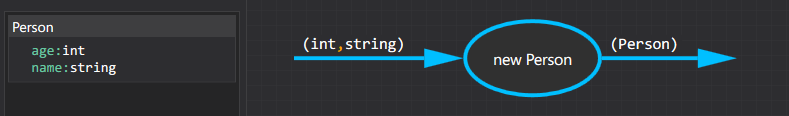
\includegraphics[width=\linewidth]{./img/roslyn_simpleOutput.png} 
		\caption{Dexel-Screenshot: Einfache Funktionseinheit mit benutzerdefinierten Datentyp}
	\end{figure}

	
	Die Generierung erzeugt folgenden Code:
	\begin{lstlisting}[caption=Mit Dexel generierter Code ]
public class Person
{
	public string Name;
	public int Age;
}

public static Person NewPerson(int aint, string astring)
{
	throw new NotImplementedException();
}
	\end{lstlisting}
	
	Hat ein Output mehr als ein Datentyp und ist kein Stream und ist auch nicht optional, so
	wird das Ergebnis als Tupel über den Rückgabewert geliefert.
	
		\begin{figure}[H]
			\centering
			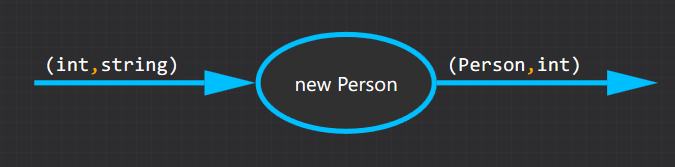
\includegraphics[width=.8\linewidth]{./img/roslyn_twoDatatypesOneOutput.png} 
			\caption{Dexel-Screenshot: Funktionseinheit mit Tupel-Output}
		\end{figure}

	
	
	\begin{lstlisting}[caption=Mit Dexel generierter Code ]
public static Tupel<Person, int> NewPerson(int aInt, string aString)
{
	throw new NotImplementedException();
}
	\end{lstlisting}

	
\subsubsection{Outputs über Actions}

	Ob ein Ausgang über ein Action realisert wird, wird indirekt dadurch
	festgelegt, dass ein Actionname angegeben wurde \footnote{Diese Regel wurde im
		Rahmen dieser Anwendung so festgelegt}. 
	
	Ausgänge müssen nicht zwingend mit
	der Anzahl an Aufrufe der Funktionseinheit übereinstimmen. Ein Action muss
	nicht aufgerufen werden, oder kann bei einem einzigen Aufruf der Funktionseinheit auch
	mehrmals aufgerufen werden (der Beginn eines Streams). 
	
	Sobald auch eine Funktionseinheit mehrere Ausgänge hat, diese jedoch nicht
	Optional sind, werden diese jedoch trotzdem als Actions realisiert, selbst wenn sie kein
	Actionname zugeordnet bekommen haben. Der Name des Actions wird dann
	automatisch generiert\footnote{	Durch Analyse der Datentypen. Ein
	(Person) wird dann zu einem onPerson. Ein () wird zu einem continueWith}.
	
	Durch diese Entscheidungen gibt es keine invaliden Kombinationen an
	Ausgängen einer Funktionseinheit.
	
	
	Werden alle Ausgänge mit Actions realisiert, entfällt der Rückgabewert in diesem Fall komplett.
	
	Die Input-Daten werden in der Signature zuerst aufgelistet, anschließend die Actions.
	
			\begin{figure}[H]
				\centering
				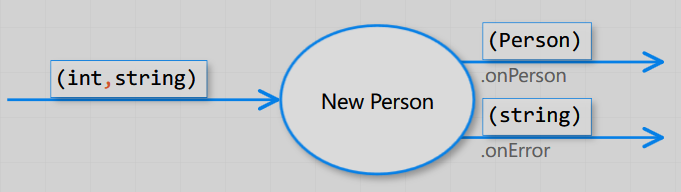
\includegraphics[width=\linewidth]{./img/roslyn_multipleOutputs.png} 
				\caption{Dexel-Screenshot: Funktionseinheit mit zwei Outputs mit definierten Actionnamen}
			\end{figure}
			
	

	
	\begin{lstlisting}[caption=Mit Dexel generierter Code ]
	public static void NewPerson(int aint, string astring, Action<Person> onPerson, Action<string> onError)
	{
	throw  new NotImplementedException();
	}
	\end{lstlisting}
	 \subsubsection{Streams}

	Streams werden in Dexel ebenfalls mit Actions realisiert, mit einer Ausnahme:
	
	Sind ist sowohl der Input als auch der Output ein Stream und ist der \textit{Actionname} dieses Outputs \textit{nicht} angegeben, so wird  implizit davon ausgegangen, dass für jeden Aufruf der Funktionseinheit dieser Output erzeugt wird. 
	
	Somit kann für diesen Output auf eine Action verzichtet werden und der Rückgabewert genutzt werden, was eine einfachere Verwendung dieser Funktionseinheit im Code zur Folge hat.
	\footnote{	Das Vorhandensein von einem Inputstream und einem Outputstream bedeutet eigentlich nicht zwingend , dass für jeden Input auch ein	Output erzeugt wird. Die Notation unterscheidet beide Fälle nicht. Deswegen die Lösung über eine Vergabe eines \textit{Actionamen} als Kompromiss, um dem Benutzer hier eine Kontrolle über die Erzeugung des Codes zu geben. Wenn der Benutzer ein \textit{Actionname} angibt, wird also indirekt davon ausgegangen, dass der Benutzer den Output auch als Action umsetzten möchte und die Funktionseinheit somit beliebig oft diese Action aufrufen kann. Ob dieses Entscheidung richtig war müsste  noch in der Praxis erprobt werden. Stellt sich heraus,	dass sie schlecht ist, müsste man über eine Anpassung der Notation nachdenken.}
	
		
		\begin{figure}[H]
			\centering
			\includegraphics[width=.9\linewidth]{./img/roslyn_Stream.png} 
			\caption{Dexel-Screenshot: Funktionseinheit mit Output-Stream}
		\end{figure}
		
	

	
	
\begin{lstlisting}[caption=Mit Dexel generierter Code ]
public static void NewPersons(int aInt, string aString, Action<Person> onPerson)
{
	throw new NotImplementedException();
}
\end{lstlisting}
	
		
	\begin{figure}[H]
		\centering
		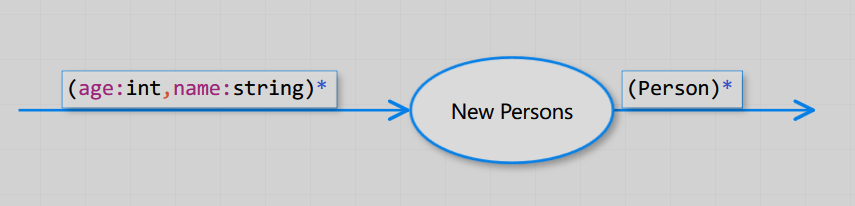
\includegraphics[width=.9\linewidth]{./img/roslyn_StreamStream.png} 
		\caption{Dexel-Screenshot: Funktionseinheit mit Input-Stream und Output-Stream und undefinierten Actionnamen}
	\end{figure}
			

	\begin{lstlisting}[caption=Mit Dexel generierter Code ]
public static Person NewPersons(int age, string name)
{
	throw new NotImplementedException();
}
	\end{lstlisting}
	 

\subsection{Erzeugung der Integration-Bodys}
\label{sec:orgheadline51}


	 \subsubsection{Terminologie}

	Eine Integration kann nicht nur aus
	Operationen bestehen, sondern auch aus anderen Integrationen bestehen.
	Leider gibt es hierfür keine Überbegriff für beide.
	Da im in diese Kapitel jedoch öfters von Funktionseinheiten innerhalb einer
	Integration die Rede sein wird, muss hierfür ein Überbegriff eingeführt
	werden. Funktionseinheiten, die sich in einer Integration befinden, werden
	nachfolgend als Sub-Funktionseinheiten bezeichnet.
	
	\subsubsection{Die Herangehensweise}

	
	Die automatische Erzeugung eines Integration ist die komplexeste Aufgabe in
	diesem Projekt. Um die Aufgabe überschaubar zu halten, wurde diese im Groben in
	zwei Teileaufgaben zerteilt: die Analyse und die Generierung.
	Die Analyse besteht wiederum aus unterschiedlichen Methoden, die jeweils das
	Flow Design auf eine bestimme Sache analysieren und das Ergebnis in ein Objekt
	abspeichern. Diese Objekt wurde als \texttt{IntegrationBody} bezeichnet.
	Diese beinhaltet alle Informationen aus der Analyse. Am Ende wird dieses Objekt
	der Generierungsmethode Übergeben, die anhand diesem den Code erzeugt\footnote{Ein weiterer Vorteil dieser Aufteilung ist, dass ein großer Teil frei von der Roslyn-API bleibt. Die eigenen Datentypen lassen sich dazu auch besser testen, als die SyntaxNodes von Roslyn. Möchte man das Ergebnis von Roslyn testen, bleibt einem  oft keine andere Wahl, als den erzeugten Code samt Whitespaces über ein string-Vergleich zu erschlagen, was bei mehrzeiligem Code doch etwas ausufern kann. Stattdessen lässt sich das Ergebnis aus den eigenen Analysen hingegen einfach über ein Vergleich von den gefundenen Objekt-Referenzen überprüfen.}.
	
	\begin{lstlisting}[caption=GenerateIntegrationBody Methode]
public static SyntaxNode[] GenerateIntegrationBody( SyntaxGenerator generator, MainModel mainModel, FunctionUnit integration )
{
	// integrationbody object for storing analysed and generated information
	var integrationBody = IntegrationAnalyser.CreateNewIntegrationBody( mainModel.Connections, integration);
	AddIntegrationInputParameterToLocalScope(integrationBody, integration);
	
	// analyse data flow before generation 
	IntegrationAnalyser.AnalyseParameterDependencies( integrationBody);
	IntegrationAnalyser.AnalyseLambdaBodies( integrationBody, mainModel);
	IntegrationAnalyser.AnalyseMatchingOutputOfIntegration( integrationBody, mainModel);
	IntegrationAnalyser.AnalyseReturnToLocalReturnVariable( integrationBody, mainModel);
	
	// generation
	var result = new List<SyntaxNode>();
	integrationBody.Generator = generator;
	GenerateBody(integrationBody, result.Add);
	
	return result.ToArray();
}
	\end{lstlisting}
	
	\subsubsection{Analyse des Flow Designs}

	\begin{enumerate}
		\item \texttt{AnalyseParameterDependencies}

		Da die Pipe-Notation unterstützt wird, reicht es nicht einfache aus die Daten
		aus den Datenflüssen zu nehmen, die direkt in die akutelle
		Funktionseinheit fließen. Stattdessen muss der Fluss rückwärts
		traversiert werden und auf Übereinstimmungen untersucht werden.
		Für jede Sub-Funktionseinheit muss diese Analyse durchgeführt werden.
		Für jeden Input-Datentyp jeder Funktioneinheit wird das Ergebnis gespeichert. Das Ergebnis beinhaltet ob der Datentyp überhaupt gefunden
		wurde, ob er im Input der Integration gefunden wurde, oder ob er aus einer
		anderen Sub-Funktionseinheit innerhalb des Datenflusses stammt. 
		Außerdem wird die gefundene DataStreamDefinition gespeichert, in der die
		Daten gefunden wurden. Ein Aufruf einer Sub-Funktionseinheit kann nur generiert werden, wenn alle Datentypen gefunden
		wurden.
		
		\item \texttt{AnalyseLambdaBodies}

		Manche optionale Datenflüsse oder Stream werden über Actions realisiert.
		Das bedeutet, dass sich alle nachflogenden Funktionseinheiten innerhalb
		des Lambda-Ausdruckes befinden müssen. Die Analyse speichert das Ergebnis
		in folgender Form ab. 
		
		\begin{lstlisting}[caption=LambdaBody Klasse]
public class LambdaBody
{
	public DataStreamDefinition InsideLambdaOf;
	public FunctionUnit FunctionUnit;
}
		\end{lstlisting}
		
		Da die LambdaBody-Objekte in der Reihenfolge im IntegrationBody abgelegt
		werden, in der sie im Flow Design vorkommen, kann daraus auch später die
		Reihenfolge der zu generierenden Methoden abgeleitet werden.
		
		
		Für jede Funktionseinheit wird solch ein Objekt angelegt, auch wenn es
		nicht innerhalb eines Lambdas vorkommt. Ist das der Fall, so ist der Wert
		\texttt{InsideLambdaOf} \texttt{null} . Alle Funktionseinheiten für die dieser Wert
		\texttt{null} ist, befinden sich somit direkt im Scope der Integration und nicht
		innerhalb eines Lambdas.
		
		\item \texttt{AnalyseMatchingOutputOfIntegration}

		Hat die Integration einen Output der als Action realisiert werden muss, so
		muss herausgefunden werden, welche Sub-Funkionseinheiten diesen
		Output bedienen. Dabei werden die Implementierungs-Stile der
		beiden übereinstimmenden Ausgänge mit abgespeichert. Später bei der
		Generierung gibt es somit vier Möglichkeiten:
		\begin{itemize}
			\item Beide sind Actions
			
			Die Action der Integration wird direkt an die Sub-Funktionseinheit
			weitergereicht. Dadurch erlaubt man einer Sub-Funktionseinheit das
			Aufrufen des Ausgang der Integration.
			
			\begin{lstlisting}[caption=Action-Action-Beziehung]
// Integration
public static void Main(Action<string> onError)
{
	DoSomething(onError);
}

// Operation
public static void DoSomething(Action<string> onError)
{
	throw new NotImplementedException();
}
			\end{lstlisting}
			
			
			\item Integrationsausgang ist Action, Sub-Funktionseinheitsausgang ist
			Returnwert 
			
			Die Action wird aufgerufen mit dem Methodenaufruf als Parameter.
			
\begin{lstlisting}[caption=Action-Return-Beziehung]
public static void CreateRandomPersons(int customerCount, Action<Person> onPerson)
{
	CreateNewPerson(customerCount, p => {
		var rndP = AddRndNameAndRndAge(p);
		onPerson(AddRndBudget(rndP));
	});
}
\end{lstlisting}
			\item Integrationsausgang ist Returnwert, Sub-Funktionseinheitsausgang ist
			Action.
			
			Eine lokale Variable muss vorher angelegt werden und mit \texttt{null}
			initalisiert werden. Danach wird innerhalb des Lambas des Actions diese
			Variable beschrieben. Am Ende wird die lokale Varibale als Rückgabewert
			ausgegeben.
			
\begin{lstlisting}[caption=Return-Action-Beziehung]
public static void TryGetMessage(Action<string> onError)
{
	throw new NotImplementedException();
}

public static string Main()
{
	string @return = null;
	TryGetMessage(msg =>  @return = msg );
	return @return;	
}
\end{lstlisting}

			\item Beide Ausgänge werden über Returnwert realisiert
			
		    Das Ergebnis der Sub-Funktionseinheit wird durch ein return-Ausdruck aus der Integration herausgereicht.
		    
\begin{lstlisting}[caption=Return-Return-Beziehung]
public static string GetMessage()
{
	throw new NotImplementedException();
}

public static string Main()
{
	var msg = GetMessage();
	return msg;
}
\end{lstlisting}		    
		    
		\end{itemize}
			\item \texttt{AnalyseReturnToLocalReturnVariable}
			
			Wird der Ausgang einer Integration mit dem Returnwert realisiert, so muss noch herausgefunden werden, ob eine lokale Variable nötig ist, um den Returnwert aus
			einem Lambda herauszureichen. Ist eine Return-Return Beziehung vorhanden und befindet sich die betroffene Methode innerhalb eines Lambda-Ausdrucks, so muss der Returnwert in die lokale \texttt{@return}-Variable geschrieben werden.
	\end{enumerate}
	



\section{Generierung eines Diagrammes aus Code}

Aus zeitlichen Gründen, konnte die Generierung von einem Flow Design aus Code nicht angegangen werden. 
Da sich das Model jedoch sauber getrennt von der GUI in
einem speraten Unterprojekt befindet, wäre es sicherlich möglich einen anderen
Studenten dies als Bachelorarbeit zu übergeben. So hätte dieser bereits eine
Möglichkeit seine Diagramme darzustellen, ohne sich sonderlich in die
Codebasis von dem gesamten Dexel-Projektes einarbeiten zu müssen.

	
	\bookmarksetup{startatroot}% this is it
	\addtocontents{toc}{\bigskip}% perhaps as well
	
	
	
		
	%%%%%%%%%%%%%%%%
	% Außerhalb von TEIL 2
	%%%%%%%%%%%%%%%%

	\chapter{Zusammenfassung}
\section{Ausblick}
Hier eine Auflistung dessen, was aus zeitlichen Gründen noch nicht realisiert
wurde, jedoch für den Einsatz in einem Projekt noch sehr wichtig wären.
Diese hat keinen Anspruch auf Vollständigkeit.
\subsubsection{Editor}
\begin{itemize}
	\item Joined-Inputs und auch Split Outputs. Dies erfordert Möglicherweise noch einmal
	eine kleine Überarbeitung des Domänenmodells. Auch die Darstellung wurde noch nicht realisiert. Zusätzlich wird die Generierung etwas komplexer und wirft weitere Fragen auf eine eindeutige Interpretation auf.
	
	\item Validierung der Syntax - Markierung invalider Syntax innerhalb des Editors wurden nicht realisiert (z.B sind die Klammern richtig gesetzt).
	
	\item Search-Replace Funktionalität, um Datentypen oder andere Namen, die an vielen Stellen verwendet werden, schnell und  einfach umbenennen zu können.
	
	\item Mehr Möglichkeiten die Darstellung übersichtlicher zu gestalten: Auf und
	Zuklappen von Integrationen. Eine 'referenzierte' Kopie einer
	Funktionseinheit zu erstellen, um an anderer Stelle diese weiter zu
	verwenden.
	\item Saubere und eindeutige Darstellung einer Rekursion.
	\item Zuordnen von Funktionseinheiten zu Klassen.
	\item Möglichkeit mehrere Flow Design in einer Art Projekt zu Organisieren.
	Vielleicht auch in Form eines GUI-Skizzen-Editors, indem dann die
	Interaktionen eingetragen werden können.
	\item Autosave und Undo/Redo.
	\item Eine Möglichkeit große unüberschaubare Flow Designs in kleinere aufzuteilen und diese an anderen Stelle zu definieren.
	
\end{itemize}


\subsubsection{Generierung von Code}
\begin{itemize}
	\item Übergabe einer Eigenschaft eines Objektes an eine Funktionseinheit.
	Bsp: product.Price -> CalculateDicount -> ...				 
	\item Zusammenführen von Datenströmen (Joined Inputs), in manchen Fällen fördert dass die Leserlichkeit.
	\item Weitere Möglichkeiten einführen um die Daten auf den Datenflüssen kurz und leserlicher zu halten.
	Zum Beispiel indem man  Aliase für Typen definieren kann, sodass man statt \texttt{breiten:int*} auch einfach nur \texttt{breiten} schreiben kann. 
	\item Registrieren  von neuen bekannten Datentypen, sodass diese nicht als \enquote{missing Datatypes} angezeigt werden und auch nicht 
	generiert werden, falls man diese doch in Dexel definiert.
	Wenn zum Beispiel aus einer externen Bibliothek  Klassen benutzt werden.
	\item Erkennen von vorhandenen Methoden aus der Standardbibliothek/LINQ, sodass für diese keine neuen Methoden erzeugt werden.
	Auch hier müsste man dann eine Notation einführen, um ausdrücken zu können, dass eine Methode des Objekts aufgerufen werden soll und nicht einer Methode das Objekt übergeben werden soll.	
\end{itemize}


\section{Fazit}

\subsubsection{Flow Design}
Mir persönlich gefällt IOSP sehr gut. Nach einer Eingewöhnungszeit lernte ich die Lambda-Schreibweise lieben und finde sie nun auch sehr leserlich. Der Code der sonst in vielen Unterfunktionen versteckt ist, kann so auf einen Blick überschaubar gehalten und trotzdem bleibt die Abstraktionsebene hoch. Ab einer gewissen Tiefe ist eine Aufteilung in unterschiedliche Methoden jedoch trotzdem sinnvoll.

Den Vorteil von entkoppelten Methoden lernte ich bereits im Dexel Projekt kennen. Methoden können leichter angepasst werden und an unterschiedlichen Stellen verwendet werden. Die Aufgabe einer Operation ist klar definiert, was sie einfacher zu implementieren und besser testbar macht. 

Die Tatsache, dass dadurch die Integrationen frei von Kontrollstrukturen bleiben finde ich auch gut. 
Leider gilt die Aussage, das die Integrationen dadurch leicht zu verstehen bleiben, da sie frei von \enquote{Logik} bleiben leider nicht immer. Wenn eine Operation zwei oder mehrere Ausgänge hat und diese in der Integration \enquote{verdrahtet} werden, so landet doch eine gute Portion Logik auch in den Integration und dadurch wird diese auch schwerer zu verstehen. 
Trotzdem würde ich weiter diese Art bevorzugen. Falls es mal nicht so sein sollte, steht es einem schließlich auch frei an jenen Stellen von der Regel abzuweichen.


Leider scheint diese Art zu programmieren  vorerst stark auf C\# ausgerichtet zu sein. In anderen Programmiersprachen, die ich kenne - wie Java und Python - besitzen diese nicht alle Funktionalitäten, die eine Umsetzung so leserlich erlauben, wie C\# \footnote{Möglicheweise gibt es andere Programmiersprachen, die es genauso gut oder vielleicht sogar noch besser ermöglichen, jedoch kenne ich persönlich aktuell keine }.
Fehlendes Closure für Lambdas ( in Python keine mehrzeiligen Lambda-Asdrücke)innerhalb eines Lambdas. 
Auch sind Java8 Streams lange nicht so mächtig und ausgereift wie LINQ. \footnote{Diese Aussage beruht darauf, dass LINQ in so gut wie jedem C\# Projekt an sehr vielen Stellen im Code zum Einsatz kommt, Java 8 Streams hingegen werden von den meisten Java-Entwickler gemieden, weil sie eben nicht so ausgereift sind. ( Laut Aussage von Kevin Erath über seine persönlichen Erfahrungen mit Java-Entwicklungsteams innerhalb der Firma)}

Leider habe bei der Umsetzung von IOSP innerhalb von Dexel so gut wie nie auf eine Flow Design Diagramm zurückgegriffen, stattdessen habe ich es innerhalb der IDE \enquote{herunterprogrammiert} und anschließend refaktorisiert. Das mag vor allem daran liegen, dass mir eine IDE durch Intellisense oft viel Arbeit erspart, gerade wenn bereits eine große Codebasis vorhanden ist.
Mit Intellisense kann ich bereits vorhandene Methoden auffinden und bekomme angezeigt, welche Parameter diese erwarten.
Auch die Eigenschaften eines Objektes mit werden mir übersichtlich angezeigt.
All das habe ich auf dem Papier ( oder auch im aktuellen Stand von Dexel nicht).



\subsubsection{Dexel}

Wie bereits erwähnt, habe ich beim Programmieren noch nicht so oft das Bedürfnis verspürt eine Flow Design Diagramm zu erstellen, wodurch ich mir die Sinnhaftigkeit eines Editors in Frage stellte.
Auch eine automatische Generierung  vollständig und ohne Fehler zu implementieren ist ein aufwendiges Unterfangen. Verglichen dazu ist der gewonnene Zeitaufwand  relativ gering. Die paar Zeilen der Integration kann man auch selbst relativ schnell herunter tippen, letzte Anpassungen vornehmen und dabei  auch LINQ  verwenden, um  auch komplexe Algorithmen runter zu schreiben.

 Es bedarf vielleicht erst einen perfekten Roundtrip, um eine automatische Generierung zu rechtfertigen und sinnvoll in einem Workflow mit einbinden zu können.
 
 Die Generierung könnte alternativ natürlich auf für Schulungszwecken verwendet werden, um Studenten/Entwicklern IOSP näher zu bringen.
 
Auch ein Entwurf auf dem Papier hat immer noch einen gewissen Scharm und Einfachheit, die in Dexel noch nicht erreicht wurden.
Das mag vor allem daran liegen, dass noch nicht alle Notation im Editor umsetzbar sind (Joined Inputs). 
Auch einfach Pfeile von A zu B zu zeichnen ohne auf eine für den Computer Eindeutigkeit Interpretation zu achten hat auch seine Vorteile.

Dexel hat jedoch auch schon einige Vorteile gegenüber dem Entwurf auf dem Papier. Der erste ist Geschwindigkeit. 
Namen können auf der Tastatur schneller geschrieben werden, als auf mit dem Stift. Mit Hilfe von Tastenkürzel lassen sich schnell neue Funktionseinheiten hinten anhängen und so den Datenfluss schnell herunter schreiben.

Einfaches Duplizieren des Schaubildes und vorhandene Elemente neu anzuordnen und Texte abzuändern ist ein klarer Pluspunkt für Dexel.

Auch eine Validierung des Datenflusses kann vorteilhaft sein.



Der aktuelle Stand ist denke ich trotzdem ein guter Start geworden, der eine Vision aufzeigt, wie ein Editor für Flow Design aussehen könnte.
Mir persönlich fällt es schwer anhand des aktuellen Stand des Projektes abzuschätzen, ob ein vollausgereifter Editor nicht doch einen  Platz finden könnte im \enquote{Werkzeugkasten} eines Softwareentwicklers.
 Es würde trotzdem noch einige Monate an in Anspruch nehmen,  um auf einen Stand zu kommen mit dem man sinnvoll Arbeiten kann und erst dann lässt sich sagen, wie sinnvoll er im Einsatz eines Softwareprojektes wirklich ist.
  Vielleicht ergibt es sich die Möglichkeit  im Rahmen einer Masterarbeit daran weiter zu arbeiten. Vielleicht findet sich auch  ein anderer Student, der bereit ist, sich in ein bestehendes Projekt einzuarbeiten und im Rahmen seiner Bachelorabeit daran weiterarbeiten möchte.



	
						
	
\chapter{Appendix}
\section{Tabstopp-Logik}


Dieses Beispiel zeigt noch einmal, dass Coderedundanzen innerhalb
von mehreren Integrationen nichts Schlechtes sein muss.

Außerdem macht es auch deutlich, wie eine etwas komplexerer Integration mit
mehreren verschachtelten Lambda-Ausdrücken in der Praxis aussehen kann.

Mit Tab und Shift-Tab ist es dem Nutzer möglich den Tastaturfokus zu
verändern

Der nächsten Tabstopp soll nach folgenden Regeln und abhängig vom aktuell
fokussierten \textit{Model} bestimmt werden:

\begin{enumerate}
	\item FunctionUnit
	
	Besitzt aktuell die View einer FunctionUnit den Tastaturfokus, so soll als
	nächster Tabstopp der erste Datenfluss, der verbunden ist gewählt werden. Ist keiner
	verbunden, wähle als nächsten Tabstop den ersten Ausgang der Funktionseinheit.
	
	\begin{figure}[H]
		\centering
		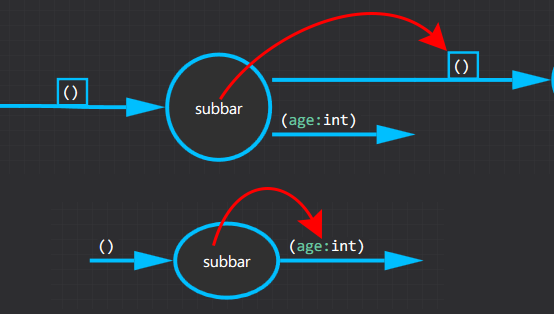
\includegraphics[width=0.6\linewidth]{./img/tabstop_functionunit.png}
		\caption{Aufgabe - Tabstopp von FunctionUnit aus}
	\end{figure}
	
	\item DataStream
	
	Wenn der Fokus aktuell auf einem DataStream liegt, so ist der nächste Tabstopp die Ziel-Funktionseinheit des Datenflusses.
	
	\begin{figure}[H]
		\centering
		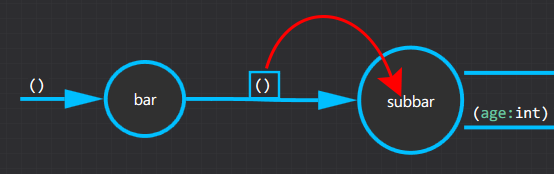
\includegraphics[width=0.6\linewidth]{./img/tabstop_datastream.png}
		\caption{Aufgabe - Tabstopp von DataStream aus}
	\end{figure}
	
	\item DataStreamDefinition
	
	Der komplexeste Fall: 
	Zu erst muss überprüft werden, ob es sich um ein Eingang oder Ausgang
	handelt. Ist es ein Eingang (A), so soll als nächster Tabstopp die Funktionseinheit
	zurückgegeben werden, von der die DataStreamDefinition der Eingang ist. 
	Bei einem Output muss überprüft werden, ob das Ende des Flows erreicht
	wurde, oder nicht. Wird ein verbundener Output entdeckt, wird der
	entsprechende DataStream als nächster Tabstopp zurückgegeben (B). Ist das Ende
	erreicht, so soll zum Anfang des kompletten Flows gesprungen werden (C).
	
	
	\begin{figure}[H]
		\centering
		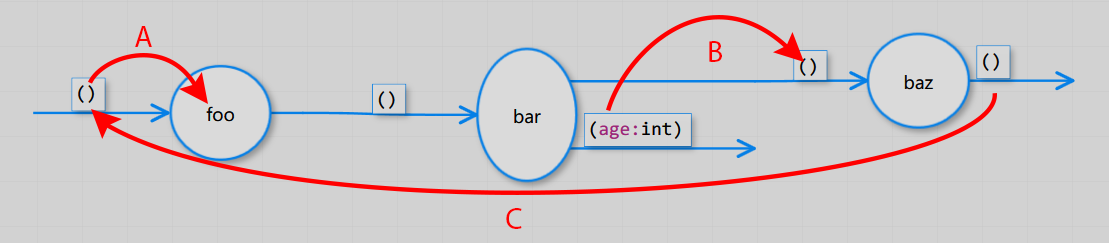
\includegraphics[width=\linewidth]{./img/tabstop_datastreamdefiniton.png}
		\caption{Aufgabe - Tabstopp von DataStreamDefinition aus}
	\end{figure}
	
	\begin{lstlisting}[caption=Tabstopp vorwärts]
	public static object TabStopGetNext(object focusedModel, MainModel mainModel)
	{
	object @return = null;
	
	focusedModel.TryCast<FunctionUnit>(fu =>
	{
	// prefer connected outputs as next tabstop
	// if no connected take first output defintion if there are any
	fu.OutputStreams.GetFirstConnected(
	foundConnected: connectedDsd => 
	@return =MainModelManager.FindDataStream(
	connectedDsd, mainModel),
	noConnected: () => 
	@return = fu.OutputStreams.FirstOrDefault());
	});
	
	focusedModel.TryCast<DataStream>(stream =>
	{
	// if focus was inside datastream take its destination function unit as next tabstop
	if (stream.Destinations.Any())
	@return = stream.Destinations.First().Parent;
	});
	
	focusedModel.TryCast<DataStreamDefinition>(dsd =>
	{
	// if focus was inside definition there are two case:
	// is input definition: next tabstop is the function unit of the definition
	// is output definition: in case the end of the flow was reached ( no connected output ) 
	// the next tabstop is the first input definition of the beginning of the whole flow.
	// Is the end not reached go to first connected output datastream
	dsd.CheckIsInputOrOutput( 
	isInput: () => @return = dsd.Parent,
	isOutput: () =>
	{
	dsd.Parent.OutputStreams.GetFirstConnected(
	foundConnected: connectedInput => 
	@return = MainModelManager.FindDataStream(
	connectedInput, mainModel),
	noConnected: () =>
	// loop tabstop focus when the 
	// end is reached
	@return = MainModelManager.GetBeginningOfFlow(
	dsd.Parent, mainModel)); 
	});
	});
	return @return;
	}
	
	\end{lstlisting}
	Analog dazu die Tabstopp-Methode in die entgegengesetzte Richtung.
	
	
	\begin{lstlisting}[caption=Tabstop rückwärts]
	public static object TabStopGetPrevious(object focusedModel, MainModel mainModel)
	{
	object @return = null;
	
	focusedModel.TryCast<FunctionUnit>(fu => 
	{
	fu.InputStreams.GetFirstConnected(
	foundConnected: connectedDsd => 
	@return = MainModelManager.FindDataStream(
	connectedDsd, mainModel),
	noConnected: () =>
	@return = fu.InputStreams.FirstOrDefault());
	});
	
	focusedModel.TryCast<DataStream>(stream => 
	{
	if (stream.Sources.Any())
	@return = stream.Sources.First().Parent;
	});
	
	focusedModel.TryCast<DataStreamDefinition>(dsd => 
	{
	dsd.CheckIsInputOrOutput(
	isOutput: () => @return = dsd.Parent,
	isInput: () => 
	{
	dsd.Parent.InputStreams.GetFirstConnected(
	foundConnected: connectedInput =>
	@return = MainModelManager.FindDataStream(
	connectedInput, mainModel),
	noConnected: () =>
	// loop tabstop focus when
	// the beginning is reached
	@return = MainModelManager.GetEndOfFlow(
	dsd.Parent, mainModel));
	});
	});	
	return @return;
	}
	\end{lstlisting}
	
	
	
	Auf oberster Ebene wird überprüft um welchen Typ von Objekt es sich
	handelt, der aktuell fokussiert ist \footnote{Teile davon war Aufgabe der UI und die
		Interaktion bekommt das Model dann als \texttt{object} übergeben. Deshalb bedarf es
		innerhalb der Methode einer Überprüfung des Typen mit TryCast. Natürlich
		könnte man dies auch durch ein Interface verhindern, dann würden die 3 Fälle
		jedoch nicht mehr klar vor einem liegen, sondern in den jeweiligen
		Implementierungen der Klassen versteckt.}. Nun existieren die drei Fälle, abhängig vom übergebenen Typen.\footnote{Zur Erinnerung: Die \texttt{Sources}-Eigenschaft eines \texttt{DataStream} beinhaltet nicht die Funktionseinheit,
		sondern die \texttt{DataStreamDefinition} einer Funktionseinheit. Die eigentliche
		Funktionseinheit enthält die \texttt{Parent}-Eigenschaft der \texttt{DataStreamDefinition}.
		Analog dazu enthält die \texttt{InputStream}- und \texttt{OutputStream}-Eigenschaft der
		Funktionseinheit auch nur die \texttt{DataStreamDefinition}-Objekte nicht ein \texttt{DataStream}-Objekt.
		Eine \texttt{DataStreamDefinition} kennt jedoch nicht den Datenfluss, mit dem sie
		verbunden ist. Eine Helfer-Methode der \texttt{MainModelManager}-Klasse stellt
		diese Funktionalität zum Auffinden des \texttt{DataStream} zur Verfügung.}
\end{enumerate}




	
	

	%%%%%%%%%%%%%%%%
	% Verzeichnisse
	%%%%%%%%%%%%%%%%
	
	
	%TODO Abkürzungsverzeichnis anlegen
	
	
	%TODO Clean Code Buch, CCD, Blogs, Youtube Video
	% Literaturverzeichnis
	\nocite{*}
	\clearpage
	
	\printbibliography[title={Quellenverzeichnis}]
	
	% Verzeichnis der Listings
	\renewcommand{\lstlistlistingname}{Verzeichnis der Listings}
	\lstlistoflistings % Listings-Verzeichnis

	% Abbildungsverzeichnis
	\listoffigures 

		
	%TODO Tablellenverzeichnis


\end{document}

